\documentclass[conference,a4paper]{IEEEtran}

% -------------------------
% Packages
% -------------------------
\usepackage{url}
\usepackage{hyperref}
\usepackage{xurl}
\usepackage{graphicx}
\usepackage{amssymb}
\usepackage{amsfonts}
\usepackage{algorithm}
\usepackage{algpseudocode}
\usepackage{amsmath}
\usepackage{cite}
\usepackage{amsthm}
\usepackage{microtype} 
\usepackage{array}

\newtheorem{proposition}{Proposition}

% -------------------------
% IEEE-friendly spacing tweaks (avoid manual \vspace between sections)
% -------------------------
\setlength{\textfloatsep}{8pt plus 2pt minus 2pt}
\setlength{\intextsep}{8pt plus 2pt minus 2pt}
\setlength{\floatsep}{6pt plus 2pt minus 2pt}
\setlength{\abovecaptionskip}{4pt}
\setlength{\belowcaptionskip}{0pt}
\setlength{\abovedisplayskip}{6pt plus 2pt minus 2pt}
\setlength{\belowdisplayskip}{6pt plus 2pt minus 2pt}
\setlength{\abovedisplayshortskip}{4pt plus 2pt minus 2pt}
\setlength{\belowdisplayshortskip}{4pt plus 2pt minus 2pt}

% Help prevent overfull boxes in narrow columns (mild, IEEE-safe)
\emergencystretch=1.5em

% Allow display breaks in long derivations (conservative)
\allowdisplaybreaks[2]

\ifCLASSINFOpdf
\else
\fi

\hyphenation{op-tical net-works semi-conduc-tor}

\DeclareRobustCommand*{\IEEEauthorrefmark}[1]{\raisebox{0pt}[0pt][0pt]{\textsuperscript{\footnotesize #1}}}

\begin{document}

\title{A Mathematical Framework for Temporal Modeling and Counterfactual Policy Simulation of Student Dropout}

\author{
\IEEEauthorblockN{
Rafael da Silva,
Jeff Eicher,
Gregory Longo
}
\IEEEauthorblockA{
PhD in Applied Data Science Program \\
School of Mathematics and Computational Sciences \\
Eastern University \\
St. Davids, PA, USA \\
\{rafael.dasilva, jeff.eicher, gregory.longo\}@eastern.edu
}
}

\maketitle

\begin{abstract}
This study proposes a temporal modeling framework with a counterfactual policy-simulation layer to examine student dropout in higher education using time-stamped learning-management-system (LMS) engagement data and administrative withdrawal records. Dropout is operationalized as an observed time-to-event outcome at the course-run enrollment level, and weekly risk is modeled in discrete time via a penalized, class-balanced logistic regression over weekly person--period rows. As a robustness check, we also fit a Cox proportional hazards model with time-varying covariates.

Under a late-event temporal holdout, the discrete-time model attains row-level AUCs of 0.8359 on training and 0.8396 on test for discriminating weekly hazard. Complementary ablation analyses indicate that performance and survival diagnostics are sensitive to the feature set composition, highlighting the role of temporal engagement signals in risk modeling. For decision-oriented evaluation, a structural hazard-scaling policy is examined via counterfactual simulation, producing survival contrasts $\Delta S(T)$ under explicit, auditable scenario parameters. Beyond aggregate evaluation, the framework is applied in a subgroup-sensitive analysis to compare how the same scenario changes survival gaps between groups, with uncertainty quantified via bootstrap. These results are not presented as causally identified effects, but as evidence that the mathematical framework supports structural policy evaluation and consistent scenario comparison when intervention effects are not identifiable from the available observational data.
\end{abstract}

\begin{IEEEkeywords}
student dropout, survival analysis, time-varying covariates, discrete-time hazard modeling, counterfactual policy simulation, learning analytics.
\end{IEEEkeywords}

\IEEEpeerreviewmaketitle



\section{Introduction}

Student dropout in higher education continues to impose substantial costs on individuals, families, institutions, and society. Higher-education leaders have emphasized the persistence of the problem, arguing that the core challenge is not only financing but also completion and persistence \cite{Crow2023CompletionCrisis,Shapiro2023SomeCollegeNoCredential}.

A large body of work has studied dropout prediction using machine-learning models built from demographic, academic, and engagement signals. However, many operational approaches still emphasize static, single-time risk estimates that primarily address \emph{who} is likely to drop out, offering limited resolution about \emph{when} risk intensifies over the course timeline \cite{Prenkaj2021SurveyMLDropout,AndradeGiron2023DropoutMLReview}. This mismatch often constrains institutions to reactive support or poorly timed interventions relative to the onset of disengagement. In practice, moving from prediction to action requires (i) expressing risk in temporal terms, (ii) translating temporal risk into auditable decision rules and timing, and (iii) comparing alternative support scenarios as explicit intervention regimes.

\noindent\textit{From prediction to policy.}
Static risk scores primarily indicate \emph{who} is at risk, but operational support also depends on \emph{when} risk increases and which decision rule triggers action. Once risk is expressed as a time-indexed hazard trajectory, the next step is to compare explicit intervention rules as regime scenarios (e.g., triggering criteria and short windows of hypothetical hazard reduction). Here, the policy layer is used for \emph{structural} evaluation: it contrasts survival trajectories implied by the model under alternative regimes, without claiming observational identification of causal effects.

Rather than conceptualizing dropout as a static outcome, we model withdrawal as a dynamic process unfolding over academic time. We operationalize dropout as administrative withdrawal from a course run with an observed unregistration time, enabling a time-to-event representation in discrete academic weeks. The predictive backbone is a discrete-time hazard framework fit on weekly person--period observations, with calibration to yield interpretable hazard probabilities over time.

Beyond prediction, the framework incorporates a \emph{structural counterfactual policy simulation} layer. Under explicit user-defined parameters, model-implied hazards are scaled to represent a hypothetical support regime, enabling comparison of survival trajectories across structural scenarios. In this setting, predicted hazards are interpreted as ``warning windows'' that support sensitivity analysis of intervention timing and magnitude along each enrollment trajectory, while maintaining a clear distinction between regime contrasts in model-implied risk and real-world intervention effects.

The framework \emph{can be} applied in a subgroup-sensitive way for groups defined by observable characteristics. To evaluate this capability, we apply the same simulated regime to observable groups (e.g., disability status) and examine how the regime contrast translates into changes in the survival gap between groups. This analysis does not claim causal identification of subgroup effects; instead, it demonstrates that the mathematical framework supports consistent structural policy evaluation across observable groups, which may motivate future extensions toward more targeted support design.

This study uses the Open University Learning Analytics Dataset (OULAD), which combines time-stamped virtual learning environment (VLE) interaction logs, assessment information, and administrative records \cite{Kuzilek2017OULAD}. The framework is designed to be transferable \emph{when} (i) time-stamped engagement traces and (ii) a well-defined time-to-event endpoint are available, as in many LMS and administrative contexts. In addition, the pipeline includes auxiliary checks---such as calibration/robustness diagnostics and comparison against an alternative baseline---to support empirical validation of the framework.

The paper evaluates the framework through three research questions and their corresponding empirical outputs: (i) construction of the weekly person--period dataset and the temporal split; (ii) temporal risk modeling (hazard) and calibration, producing the baseline risk and implied survival trajectory for \textbf{RQ1}; (iii) structural counterfactual policy simulation (\textbf{RQ2}); and (iv) subgroup validation via gap analysis (\textbf{RQ3}). The next section provides background on student dropout and motivates a temporal, log-based perspective in online learning settings, which sets the stage for the formal definitions and modeling introduced later.
\section{Background}
Student dropout is consequential for both learners and institutions, and its dynamics often become visible through changes in engagement across an academic term. As instruction increasingly shifts to online and hybrid formats, time-stamped learning traces make it possible to examine dropout risk with an explicitly temporal perspective.

\subsection{Why Dropout Matters: Impacts and Scale}
Student dropout has far-reaching consequences at the individual, family, institutional, and societal levels. For individuals, dropout disrupts educational attainment, limits skill development, and can negatively affect motivation and well-being. At the family level, it often represents a substantial sunk financial investment and constrains intergenerational social mobility \cite{Kamissa2020DroppingOut}. Institutions face declining program quality, reputational harm, and revenue losses from reduced enrollment and opportunity costs \cite{Guzman2021DropoutRural, Schneider2010FirstYearAttrition}.

In the United States, approximately 30\% of undergraduates drop out after their first year, resulting in over 9 billion dollars annually in public expenditures with limited social returns \cite{Schneider2010FirstYearAttrition}. Globally, despite expanded access to tertiary education, substantial dropout persists across systems as documented in socio-economic reviews \cite{Aina2022DeterminantsDropout}. Course-level dropout further increases the risk of program withdrawal, institutional exit, and reduced re-enrollment, particularly among marginalized students \cite{McKinney2019CourseDropping, Gicheva2025PersistenceIntroCourse}. These cascading effects underscore the need for early detection and timely support.

\subsection{Structural Shifts in Delivery: From Distance to Online}
Student dropout must be understood within the structural transformation of higher education delivery. Although online learning appears recent, distance education has historical roots in correspondence-based instruction and evolved into online formats with the expansion of the internet \cite{Kentnor2015DistanceEducation}. The COVID-19 pandemic accelerated this shift, forcing institutions worldwide to rapidly adopt online delivery and redefining online education as a core instructional mode rather than a supplement \cite{Bartolic2022COVIDTeaching, Bryson2020RapidAdoption, Zhang2023OnlineLearningReview}.

This transition embedded online education into institutional strategy, led to widespread program migration, and prompted substantial pedagogical redesign. Learning Management Systems (LMS) consequently became central infrastructures for teaching and engagement, generating rich, time-stamped behavioral data \cite{Turnbull2021TransitioningELearning}. These data enable temporal analytics that move dropout modeling beyond static prediction.

Dropout in online higher education reflects a distinct ``dropout ecology'' shaped by social isolation, reduced interaction, and heightened self-regulation demands \cite{Rahmani2024OnlineDropoutReview}. Attrition arises from intersecting academic, institutional, and personal barriers, including workload, financial, health, and technological constraints. While socioeconomic status and academic performance consistently predict early dropout \cite{BarraganMoreno2024ComplexitiesDropout}, comparative analyses across disciplines and study levels remain limited, with much research focused on MOOCs \cite{Prenkaj2021SurveyMLDropout,Sghir2022PredictiveLearningAnalytics,Alalawi2023MLStudentPerformance}.
Learning Management Systems enable detailed tracking of engagement, which correlates with academic outcomes \cite{Mozahem2020LMSActivity}. Although machine-learning models achieve high predictive accuracy, challenges persist due to data heterogeneity, limited reproducibility, and insufficient temporal and contextual modeling \cite{Albreiki2021MLPerformanceReview,Schneider2010FirstYearAttrition}.

\subsection{Intervention Practice Gaps: Documentation, Evaluation, and Experimental Frictions}
In many higher-education settings, intervention practices are deployed in an ad hoc manner, varying across instructors, courses, and academic terms, and are often insufficiently documented to support systematic evaluation \cite{Connolly2018TrialsEvidenceBased,Harackiewicz2018TargetedIntervention,Kizilcec2020ScalingInterventions}. The absence of structured intervention policies and consistent logging makes it difficult to determine when an intervention occurred, to whom it applied, and under which conditions \cite{Sonderlund2018LAInterventions,Page2020ClusteredObservationalEducation,Kitto2023CausalModelsLA}. As a result, routine observational data typically lack the granularity required to support credible causal evaluation of intervention effects in real-world academic operations \cite{Gallagher2020ChallengeBased,Sidiropoulos2022AgencySustainability}. Although randomized experiments (e.g., A/B testing) can, in principle, address these identification gaps, their implementation in live academic environments is frequently constrained by operational and practical considerations---such as coordination overhead, time-to-evidence, and uncertainty about where experimentation is most likely to yield actionable insights \cite{Chan2019AIMedEd,Connolly2018TrialsEvidenceBased,HahsVaughn2024MultisiteTrialChallenges}. In this setting, scenario-based structural comparison is not a substitute for causal inference, but a disciplined way to study how a fitted temporal model behaves under explicit intervention rules when intervention histories are not identifiable \cite{Igelstrom2022CausalInferenceObs,DoutreligneVaroquaux2025PredictiveDecisionCausal}.
\section{Methodology}

The framework maps temporally indexed enrollment data to weekly hazard estimates, simulated regime contrasts, and subgroup diagnostics. It combines person-period construction, leakage-aware hazard modeling, policy simulation, and subgroup analysis under explicit inferential limits.

\subsection{Motivation, Contributions, and Research Questions}

\paragraph*{Motivation.}
Static risk models primarily answer \textit{who} is at risk, but they do not by themselves determine \textit{when to act} under an auditable operational rule \cite{Prenkaj2021SurveyMLDropout,AndradeGiron2023DropoutMLReview}. In observational settings, the comparison of intervention scenarios must therefore be framed as a structural, model-implied exercise rather than as a causally identified effect estimate \cite{Connolly2018TrialsEvidenceBased,Gallagher2020ChallengeBased,Sidiropoulos2022AgencySustainability,Igelstrom2022CausalInferenceObs,DoutreligneVaroquaux2025PredictiveDecisionCausal}. This study is motivated by that gap: the need for a temporally explicit framework that links weekly risk estimation to executable policy simulation and subgroup-sensitive interpretation.

\paragraph*{Contributions.}
The framework has four components. First, it formalizes a discrete-time hazard pipeline for estimating survival trajectories from temporally indexed student records. Second, it introduces a policy simulation layer that compares \textit{shock} and \textit{stateful mechanism-aware} regimes under a common intervention rule. Third, it adds a subgroup fairness layer to quantify how the same policy changes outcome gaps across observable groups. Fourth, it specifies an executable protocol grounded in the notebook implementation and exported artifacts.

\paragraph*{Research Questions.}
RQ1 asks whether the temporal model produces weekly hazard estimates that are sufficiently discriminative and calibrated to support decision-making. RQ2 asks what structural survival contrast emerges between simulated regimes under an explicit policy rule. RQ3 asks whether the same policy changes subgroup gaps, and with what uncertainty.

\paragraph*{Propositions.}
\begin{proposition}[Temporal bridge]
If $\hat h_{it}$ is estimated on person-period data without temporal leakage, then $\hat S_i(t)$ defines candidate temporal risk windows for downstream analysis.
\end{proposition}

\begin{proposition}[Regime contrast]
Under a fixed policy contract,
\begin{equation*}
\Delta S(t)=\bar S^{(1)}(t)-\bar S^{(0)}(t)
\end{equation*}
defines a structural contrast between simulated regimes.
\end{proposition}

\begin{proposition}[Subgroup heterogeneity]
When the same policy is applied to observable groups,
\begin{equation*}
\Delta Gap(t)=Gap^{(1)}(t)-Gap^{(0)}(t)
\end{equation*}
quantifies the differential change in trajectories under the same simulation engine.
\end{proposition}

\subsection{Notation and Evaluation Horizons}

Table~\ref{tab:method_notation} summarizes the notation used throughout the methodological tracks.

\begin{table}[!t]
\centering
\footnotesize
\renewcommand{\arraystretch}{1.05}
\begin{tabular}{@{}p{0.25\columnwidth} p{0.67\columnwidth}@{}}
\hline
Symbol & Definition \\
\hline
$i$ & enrollment (unit of analysis) \\
$t$ & discrete week \\
$X_{it}$ & observed covariates at time $t$ \\
$E_i$ & primary event indicator \\
$C_i$ & censoring time \\
$\hat h_{it}$ & predicted weekly hazard \\
$\hat S_i(t)$ & predicted survival \\
$\bar S^{(a)}(t)$ & mean survival under regime $a$ \\
$\Delta S(t)$ & structural survival contrast \\
$Gap^{(a)}(t)$ & between-group gap under regime $a$ \\
$\Delta Gap(t)$ & change in gap between regimes \\
$T_{policy}$ & primary substantive reporting horizon \\
$T_{eval\_policy}$ & temporal support evaluated in policy simulation \\
$T_{eval\_metrics}$ & stable horizon for IPCW-based metrics \\
$g_{min}$ & minimum stability threshold for $\hat G(t)$ \\
\hline
\end{tabular}
\caption{Main notation used throughout the Methodology section.}
\label{tab:method_notation}
\end{table}

The protocol distinguishes between substantive and technical horizons:
\begin{equation*}
T_{eval\_metrics}=\max\{t:\hat G(t)\ge g_{min}\},
\end{equation*}
where $T_{policy}$ denotes the main reporting horizon and $T_{eval\_policy}$ denotes the temporal support over which simulated regime trajectories are evaluated. Policy interpretation and censoring-weighted metric stability do not necessarily operate on the same horizon.

In the current exported protocol, these horizons are fixed as $T_{policy}=18$, $T_{eval\_policy}=38$, and $T_{eval\_metrics}=37$, with $g_{min}=0.05$ recorded as the operational stability threshold in the evidence package.

\subsection{Analytical Tracks}

The framework spans the bridge
\texttt{temporal hazard $\rightarrow$ survival trajectories $\rightarrow$}
\texttt{policy simulation $\rightarrow$ subgroup diagnostics}.
The implemented tracks are:
\begin{enumerate}
\item temporal pipeline and data construction;
\item leakage prevention and temporal splitting;
\item censoring and IPCW;
\item primary discrete-time hazard model (RQ1);
\item benchmark model family;
\item policy simulation (RQ2);
\item subgroup fairness diagnostics (RQ3).
\end{enumerate}

The framework does not identify causal effects from observational exposure. It defines the modeling and simulation machinery under which later contrasts are generated and interpreted.

\subsection{Problem Setup and Unit of Analysis}

The unit of analysis is enrollment $i$ observed over discrete weekly time $t$:
\begin{equation*}
i \in \{1,\dots,N\}, \quad t \in \{0,\dots,T\}, \quad X_{it}\in\mathbb{R}^p.
\end{equation*}

The analytical table is constructed in person-period format, with one row per enrollment-week. This representation is required because the target quantity is not a single static outcome per student, but a time-indexed conditional event risk that evolves over the observed trajectory.

\subsection{Primary Endpoint and Censoring}

The primary event is administrative withdrawal, operationalized as \texttt{Withdrawn} with a valid \texttt{date\_unregistration}. Cases labeled \texttt{Withdrawn} without a valid date are treated as censored under the primary endpoint definition.

\begin{equation*}
\begin{aligned}
E_i=\mathbb{1}\{&\texttt{final\_result}_i=\texttt{Withdrawn} \\
&\land\ \texttt{date\_unregistration}_i\ \text{is valid}\}.
\end{aligned}
\end{equation*}

\begin{equation*}
t_i^{event}=\left\lfloor \frac{\texttt{date\_unregistration}_i}{7} \right\rfloor \quad (E_i=1)
\end{equation*}

\begin{equation*}
t_i^{final}=\begin{cases}
t_i^{event}, & E_i=1, \\
t_i^{last\_obs}, & E_i=0.
\end{cases}
\end{equation*}

For non-events, $t_i^{last\_obs}$ is operationalized as the last observed VLE week and should be interpreted as an observation proxy rather than an administrative censoring timestamp.

Events are counted only when administrative timing is observed and compatible with the weekly survival setup.

\subsection{Person-Period Construction and Terminal Label}

Each enrollment is expanded weekly up to $t_i^{final}$, yielding one terminal event label at most:
\begin{equation*}
event_{it}=\mathbb{1}\{E_i=1 \land t=t_i^{final}\}
\end{equation*}

\begin{equation*}
\sum_{t=0}^{t_i^{final}} event_{it} \le 1.
\end{equation*}

This construction yields a longitudinal risk set for each enrollment and, if applicable, a single terminal event week.

\subsection{Temporal Covariate Engineering}

Dynamic covariates are defined on a weekly grid under temporally safe logic:
\begin{equation*}
w(d)=\max\left(\left\lfloor d/7 \right\rfloor,0\right)
\end{equation*}

\begin{equation*}
A_{it}=\mathbb{1}\{\texttt{total\_clicks}_{it}>0\}
\end{equation*}

\begin{equation*}
Recency_{it}=\begin{cases}
0, & A_{it}=1, \\
Recency_{i,t-1}+1, & A_{it}=0
\end{cases}
\end{equation*}

\begin{equation*}
Streak_{it}=\begin{cases}
Streak_{i,t-1}+1, & A_{it}=1, \\
0, & A_{it}=0.
\end{cases}
\end{equation*}

The main feature set includes \texttt{total\_clicks}, \texttt{recency}, \texttt{streak}, \texttt{submitted\_this\_week}, and contextual covariates. These features encode short-term engagement dynamics while preserving temporal ordering.

\subsection{Stratified Temporal Split and Leakage Prevention}

The train-test split is performed at the enrollment level, stratified jointly by event status and temporal bucket:
\begin{equation*}
time\_for\_split_i=\begin{cases}
t_i^{event}, & E_i=1, \\
t_i^{final}, & E_i=0
\end{cases}
\end{equation*}

\begin{equation*}
stratum_i=(E_i,\ bucket_q(time\_for\_split_i)).
\end{equation*}

The implemented configuration uses $q=4$ and \texttt{test\_size}=0.30. Calibration and validation procedures further use enrollment-grouped folds via GroupKFold.

The design prevents leakage across rows belonging to the same enrollment and preserves temporal composition across train and test partitions. The grouped validation logic follows the broader concern with leakage in structured machine-learning evaluation and cross-validation for dependent data \cite{KapoorNarayanan2023LeakagePatterns,RobertsEtAl2017CrossValidationEcography}.

\subsection{Primary Discrete-Time Hazard Model (RQ1)}

Following standard discrete-time event-history formulations \cite{SingerWillett1993DiscreteTimeSurvival,Allison1982DiscreteTimeMethods}, the primary modeling track estimates weekly conditional hazard and derives survival by cumulative product:
\begin{equation}
\label{eq:hazard_weekly}
h_{it}=P(event_{it}=1 \mid T_i\ge t, X_{it})
\end{equation}

\begin{equation*}
\text{logit}(\hat h_{it})=\beta_0+\beta^\top X_{it}
\end{equation*}

In implementation, the raw weekly probabilities are post-hoc calibrated through grouped sigmoid calibration (Platt scaling) to support interpretable hazard probabilities under the same enrollment-respecting split logic \cite{Platt1999ProbabilisticOutputs}.

\begin{equation}
\label{eq:survival_product}
\hat S_i(t)=\prod_{k\le t}(1-\hat h_{ik})
\end{equation}

The primary track yields weekly risk trajectories rather than a single end-of-course classification score. This layer underlies RQ1 and the downstream policy simulation.

\subsection{Censoring Track and IPCW}

The censoring component combines estimation of censoring survival with truncated inverse probability of censoring weights:
\begin{equation*}
\hat G_{it}=P(C_i\ge t \mid X_{it})
\end{equation*}

\begin{equation*}
w_{it}=\frac{1}{\max(\hat G_{it}, g_{min})}.
\end{equation*}

This weighting logic follows standard survival-prediction evaluation under right censoring \cite{Graf1999AssessmentSurvivalPrediction,Gerds2006ConsistentBrier}. The protocol separates the policy reporting horizon from the technical horizon used for censoring-weighted metrics because IPCW evaluation becomes unstable when $\hat G(t)$ is too small, even if simulated regime trajectories remain computable beyond that point. In the current protocol, $g_{min}=0.05$ yields $T_{eval\_metrics}=37$, while $T_{eval\_policy}=38$ is retained only as the raw support horizon for trajectory reporting.

Because non-event follow-up is anchored to last observed VLE activity, IPCW validity in this setup relies on conditional independent censoring given $X_{it}$ rather than unconditional random censoring. A sensitivity probe exported in \texttt{table\_censoring\_anchor\_sensitivity.csv} shows that across anchor variants the censoring-model test AUC ranges from $0.9155$ to $0.9299$, while capped-weight share in test ranges from $0.4945$ to $0.6576$ (current anchor at the upper end).

\subsection{Policy Simulation (RQ2): Shock vs. Mechanism-Aware}

The current policy contract separates external anchoring from internal scenario assumptions. The operational intervention rule is anchored to Kay and Bostock \cite{KayBostock2023PowerNudge}: ``flag if no LMS engagement in last 7 days ($\approx \text{recency} \ge 1$ week)'', with weekly checking frequency and trigger parameter $r^*=1$. This operational anchor is recorded in \texttt{table\_policy\_spec.csv}.

The active window is fixed at $W_{\text{weeks}}=2$, consistent with a short-term digital nudge framing \cite{KayBostock2023PowerNudge}. In contrast, effect intensity is treated as a scenario parameter because the observational setting does not identify a unique causal magnitude. The mechanism-aware shared schedule is frozen as $\alpha_{\text{week0}}=0.35$, $\alpha_{\text{week1}}=0.10$, \nolinkurl{decay_type=kb2023_step_2w}, and \nolinkurl{window_exclusive_upper=True}. For the shock regime, \nolinkurl{delta_shock_ablation} is reported as three scenario intensities: $0.08$ (anchored conservative scenario, qualitatively aligned with moderate intervention effects synthesized by Sneyers and De Witte \cite{SneyersDeWitte2018InterventionsMeta}), $0.20$ (hypothetical A), and $0.60$ (hypothetical B stress test).

The intervention rule is triggered by recency crossing a threshold within an activation window:
\begin{equation*}
t_i^*=\min\{t: Recency_{it}\ge r^*\}
\end{equation*}

\begin{equation*}
active_{it}=\mathbb{1}\{t\in[t_i^*,t_i^*+W)\}.
\end{equation*}

Under the \textit{shock} regime, the policy acts directly on the baseline hazard:
\begin{equation*}
\hat h^{(1,shock)}_{it}=\begin{cases}
\hat h^{(0)}_{it}(1-\delta_{shock}), & active_{it}=1, \\
\hat h^{(0)}_{it}, & active_{it}=0.
\end{cases}
\end{equation*}

Under the \textit{mechanism-aware} regime, the policy propagates through counterfactual covariate updates:
\begin{equation*}
\hat h^{(1,mech)}_{it}=f(X^{cf}_{it}).
\end{equation*}

In the mechanism-aware regime, $X^{cf}_{it}$ is updated statefully across weeks. In the exported run, the strongest perturbation channel is click-based engagement (\texttt{total\_clicks}), used as an LMS proxy analogous to participation and re-engagement dynamics discussed by Kay and Bostock \cite{KayBostock2023PowerNudge}, rather than as a literal replication of the source study variables. The shock regime applies an immediate model-level perturbation, whereas the mechanism-aware regime changes the evolving covariate path through which future hazards are generated.

Operational details of this mechanism-aware operator are exported explicitly in \nolinkurl{table_policy_mech_operator_spec.csv} (channel mode, timing, overwrite rule, and propagation rule). The schedule sensitivity battery is exported in \nolinkurl{table_rq2_sensitivity_grid.csv} and varies trigger/schedule parameters while preserving the same plug-in modeling stack used for baseline scoring.

The updated framework also keeps mechanism-aware execution auditable through run-level diagnostics exported as \nolinkurl{table_policy_activation_summary.csv}, \nolinkurl{table_policy_covariate_overwrites.csv}, and \nolinkurl{table_policy_covariate_propagation_checks.csv}, alongside the operator contract.

\subsection{Structural Survival Contrast (RQ2)}

The central policy estimand is mean survival under each regime:
\begin{equation*}
\bar S^{(a)}(t)=\frac{1}{N}\sum_i \hat S_i^{(a)}(t)
\end{equation*}

\begin{equation}
\label{eq:delta_s}
\Delta S(t)=\bar S^{(1)}(t)-\bar S^{(0)}(t).
\end{equation}
Positive values indicate a survival gain under the policy regime relative to baseline.

The interpretation of $\Delta S(t)$ is that of a \textit{simulated regime contrast} implied by the fitted model and the policy contract. It is not interpreted as a causally identified treatment effect \cite{Igelstrom2022CausalInferenceObs,DoutreligneVaroquaux2025PredictiveDecisionCausal}.

\subsection{Fairness and Subgroup Track (RQ3)}

The same policy is evaluated across observable subgroups through a gap-based contrast:
\begin{equation*}
\bar\mu_g^{(a)}(t)=\frac{1}{N_g}\sum_{i:g(i)=g}\hat S_i^{(a)}(t)
\end{equation*}

\begin{equation*}
Gap^{(a)}(t)=\bar\mu_1^{(a)}(t)-\bar\mu_0^{(a)}(t)
\end{equation*}

\begin{equation}
\label{eq:delta_gap}
\Delta Gap(t)=Gap^{(1)}(t)-Gap^{(0)}(t).
\end{equation}
The sign of $\Delta Gap(t)$ indicates whether the policy enlarges or reduces the between-group difference at the horizon of interest. Uncertainty is estimated via bootstrap, consistent with subgroup-oriented fairness auditing that reports performance and calibration gaps with interval estimates \cite{PessachShmueli2022FairnessReview,Lu2022ReliabilityFairnessAudit,Opoku2025AccuracyFairness}.

\subsection{Benchmark Track}

The benchmark track provides model-family reference comparisons without replacing the primary hazard pipeline. In the current main-text reporting, the benchmark centers on the temporal hazard model, its IPCW-weighted variant, and a non-temporal Random Survival Forest baseline at aligned horizons \cite{MogensenIshwaranGerds2012RSF}. Additional model families, including Cox time-varying specifications \cite{Cox1972RegressionModels}, can serve as auxiliary references.

\subsection{Operational Assumptions}

Interpretation rests on the following assumptions:
\begin{itemize}
\item the event and censoring definitions correctly represent the observational endpoint;
\item covariates used at week $t$ are available up to week $t$ only, with no temporal leakage;
\item policy simulation defines a model-implied structural contrast rather than a causally identified intervention effect;
\item the stability of censoring-weighted metrics is evaluated at the technical horizon $T_{eval\_metrics}$.
\end{itemize}

\subsection{Interpretive Scope}

The reported results for $\Delta S$ and $\Delta Gap$ are \textit{model-implied simulated regime contrasts}, not causally identified estimates of intervention effects.

\subsection{Reproducibility}

Code for preprocessing, temporal splitting, training and calibration, policy simulation, subgroup fairness analysis, and artifact export (\texttt{outputs\_v2}) is available at
\url{https://github.com/rafa-rodriguess/TCM-Student-Dropout}
\cite{RafaRepoTCMStudentDropout}. The reference dataset used in the pipeline is OULAD \cite{Kuzilek2017OULAD}.

The artifact package records the full policy
contract in \nolinkurl{table_policy_spec.csv}, the scenario catalog in
\nolinkurl{table_policy_scenarios_main.csv} and
\nolinkurl{table_policy_scenario_params.csv}, and scenario-resolved trajectory
outputs in \nolinkurl{table_policy_deltaS_by_week_by_scenario.csv} and
\nolinkurl{table_policy_deltaS_at_horizons_by_scenario.csv}. It also records
the dual-horizon semantics in \nolinkurl{table_policy_horizons_dual.csv}, the mechanism-aware operator contract in \nolinkurl{table_policy_mech_operator_spec.csv}, and the RQ2 schedule sensitivity grid in \nolinkurl{table_rq2_sensitivity_grid.csv}. Under the current exported protocol, these artifacts jointly encode the
anchored trigger reference, the frozen shared mechanism-aware schedule, the
anchored-vs-hypothetical shock intensity split, and the distinction between
$T_{\text{policy}}=18$, $T_{\text{eval,policy}}=38$, and
$T_{\text{eval,metrics}}=37$.
\section{Experimental Design}

This section specifies how the methodological framework was operationalized and tested to answer RQ1, RQ2, and RQ3 on the OULAD dataset. Its purpose is to define the evaluation protocol actually used, the fixed comparison rules adopted before inspecting comparative outcomes, and the evidence contract linking claims to metrics and exported artifacts. By the end of the section, the reader should expect a clear description of the cohort construction, split logic, model variants, evaluation horizons, robustness plan, and reading criteria under which the empirical results are interpreted.

This section follows the same narrative structure as the implemented pipeline. It begins with the design goals and analytical units, then defines the split and model tracks, next establishes the censoring-aware evaluation horizons and metric suite, and finally specifies the policy, subgroup, robustness, and traceability protocols. Throughout, the design is presented as a pre-specified experimental framework for evaluating \textit{model-implied simulated regime contrasts}, not as a causal identification strategy for intervention effects.

Figure~\ref{fig:pipeline_endtoend} provides an end-to-end overview of the evaluation tracks.

% Placeholder for compiled Graphviz figure (G1 pipeline_endtoend)
% To produce this figure: dot -Tpng graphviz_pipeline_endtoend.txt -o figures/fig_pipeline_endtoend.png
\begin{figure}[!t]
\centering
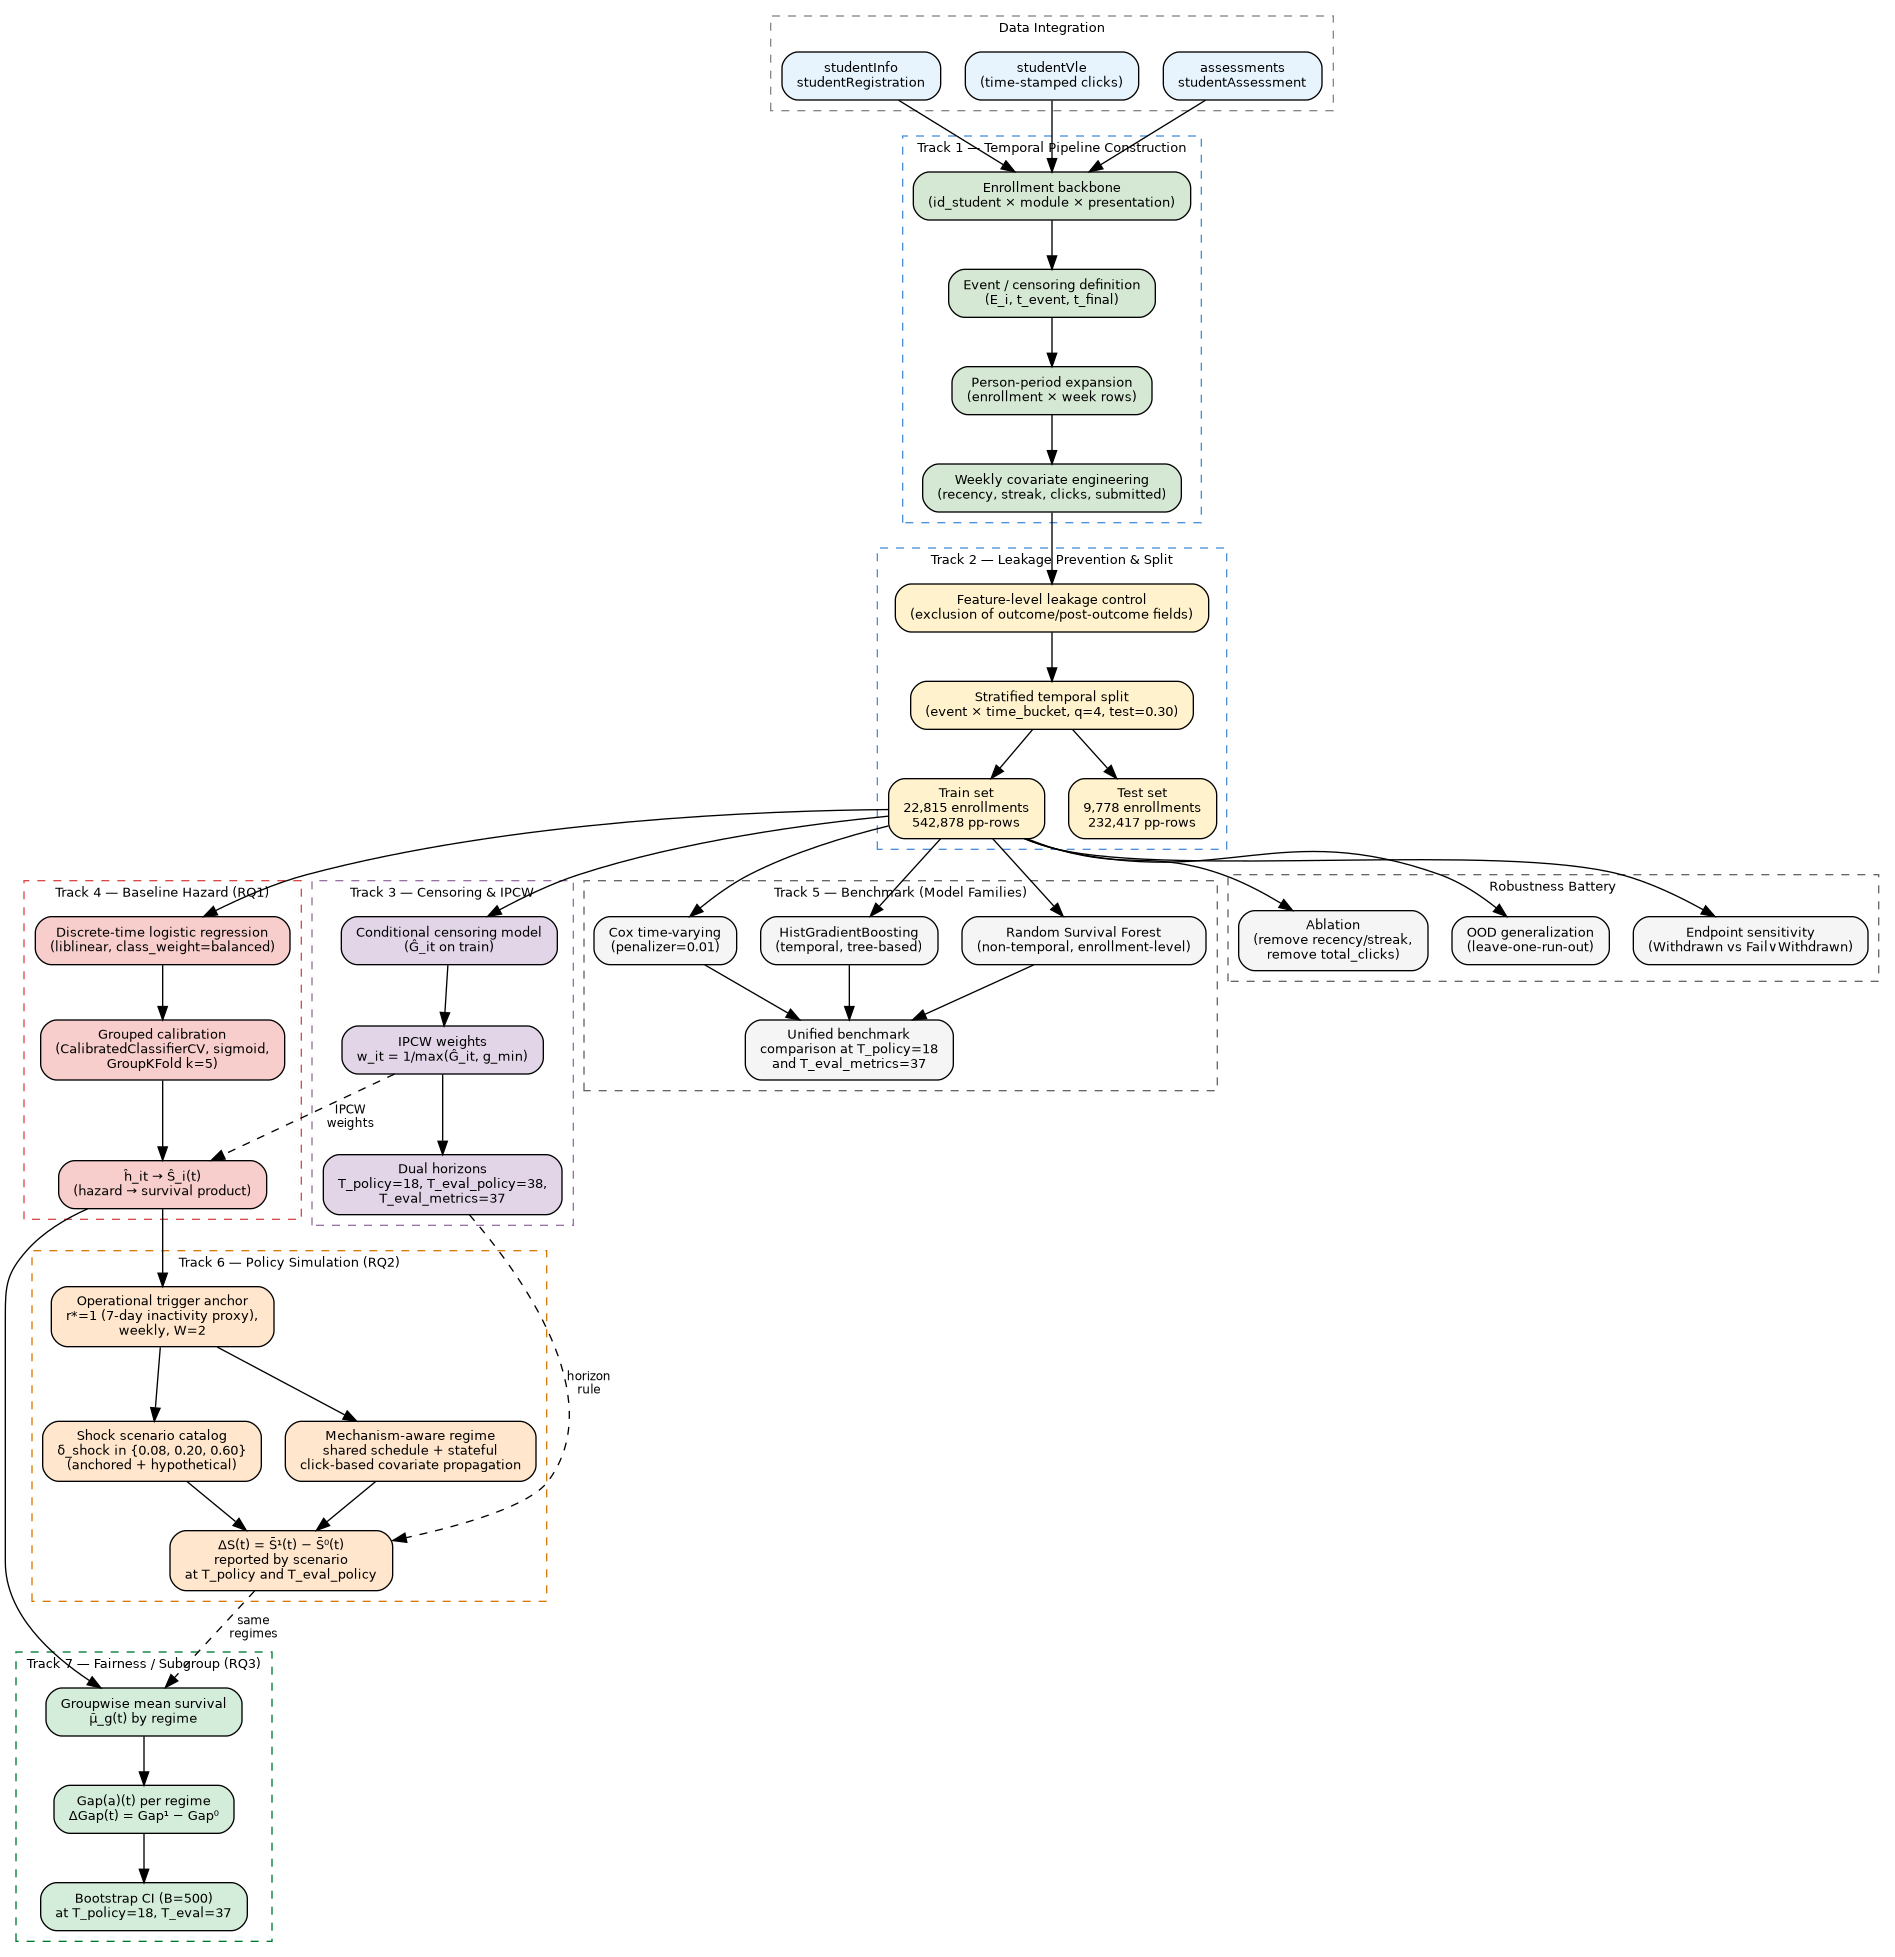
\includegraphics[width=\columnwidth]{figures/fig_pipeline_endtoend.png}
\caption{End-to-end pipeline: data integration, temporal construction, modeling, policy simulation, and fairness evaluation mapped to seven executable tracks and RQ1--RQ3, including dual-horizon semantics ($T_{policy}$, $T_{eval\_policy}$, $T_{eval\_metrics}$) and scenario-indexed shock intensity in RQ2.}
\label{fig:pipeline_endtoend}
\end{figure}

%% -----------------------------------------------------------------------
\subsection{Design Goals and Operational Research Questions}

The experimental design evaluates three core properties of the framework, each aligned with one research question and one analytical track.

\begin{itemize}
\item \textbf{RQ1 --- Temporal hazard quality.}
Does the discrete-time hazard model discriminate and calibrate well enough at the weekly person-period level to support downstream policy evaluation?

\item \textbf{RQ2 --- Structural regime contrast.}
Under an explicit deterministic Recency-triggered rule, does the aggregate structural contrast $\Delta S(t)$ (Eq.~\ref{eq:delta_s}) yield a consistent and interpretable signal at the designated reporting horizons?

\item \textbf{RQ3 --- Subgroup gap change.}
When the same rule is applied to observable subgroups, does $\Delta Gap(t)$ (Eq.~\ref{eq:delta_gap}) exhibit a direction robust to bootstrap uncertainty, thereby motivating subgroup-sensitive support evaluation?
\end{itemize}

These goals define the contract of the section. What is evaluated here is the empirical behavior of the implemented framework under fixed protocol choices. Policy and fairness outputs are therefore interpreted as \textit{simulated regime contrasts}, not as observationally identified causal effects.

%% -----------------------------------------------------------------------
\subsection{Cohort, Unit of Analysis, and Analysis Table}
\label{subsec:cohort}

\paragraph*{Data sources.}
We use the Open University Learning Analytics Dataset (OULAD)~\cite{Kuzilek2017OULAD}, integrating time-stamped VLE interaction logs (\texttt{studentVle}), assessment information (\texttt{assessments}, \texttt{studentAssessment}), and administrative enrollment records (\texttt{studentInfo}, \texttt{studentRegistration}). These sources jointly provide the temporal, assessment, and administrative components required to build a weekly enrollment-level survival dataset.

\paragraph*{Enrollment backbone.}
An enrollment is identified by the triplet $(\texttt{id\_student},\allowbreak\texttt{code\_module},\allowbreak\texttt{code\_presentation})$. After deduplication, the exported cohort contains $N=32{,}593$ enrollments from $28{,}785$ unique students. This enrollment backbone defines the analytical unit used throughout all subsequent tracks.

\paragraph*{Primary endpoint.}
Dropout requires both \texttt{final\_result = Withdrawn} and an observed valid \texttt{date\_unregistration}, yielding the indicator $E_i$ defined in Methodology. Withdrawn records without a valid unregistration date ($2{,}769$ cases) are treated as censored under the primary endpoint. This rule ensures that event counting is restricted to withdrawals with an observed administrative event time compatible with the weekly hazard formulation.

\paragraph*{Person-period table.}
Each enrollment is expanded into weekly rows $t=0,\dots,t_i^{\mathrm{final}}$ with terminal label
\[
event_{it}=\mathbb{1}[E_i=1 \wedge t=t_i^{\mathrm{final}}].
\]
This representation converts the cohort into the person-period structure required for discrete-time hazard estimation and downstream policy simulation. Table~\ref{tab:cohort_summary} reports the resulting cohort dimensions.

\begin{table}[!t]
\centering
\caption{Cohort summary: enrollment and person-period counts.}
\label{tab:cohort_summary}
\begin{tabular}{lr}
\hline
Quantity & Value \\
\hline
Enrollments ($N$) & 32{,}593 \\
Unique students & 28{,}785 \\
Withdrawn without valid date (censored) & 2{,}769 \\
\hline
\end{tabular}
\end{table}

%% -----------------------------------------------------------------------
\subsection{Stratified Temporal Split Protocol}
\label{subsec:split}

The train-test split is performed at the enrollment level to prevent row leakage across weekly observations from the same enrollment. This is a central design choice because the model is trained on person-period rows but evaluated under enrollment-level independence constraints.

\paragraph*{Stratification variable.}
We define
\begin{equation*}
time\_for\_split_i =
\begin{cases}
t_i^{\mathrm{event}}, & \text{if } E_i = 1,\\
t_i^{\mathrm{final}}, & \text{otherwise.}
\end{cases}
\end{equation*}
and then discretize this variable into $q=4$ quantile buckets. The stratum for each enrollment is
\begin{equation*}
stratum_i = (E_i,\; bucket_q(time\_for\_split_i)).
\end{equation*}
Observed bucket edges after rounding are $[0,\;8,\;31,\;34,\;63]$. This design preserves both event-status balance and coarse temporal structure across partitions.

\paragraph*{Sampling.}
Within each stratum, $30\%$ of enrollments are assigned to the test set using random seed 42, with per-stratum count clipped to $[\,1,\; n_s-1\,]$. This guarantees that each populated stratum contributes observations to both train and test whenever possible.

\paragraph*{Resulting partition.}
Table~\ref{tab:split_counts} reports the partition dimensions. All enrollment-weeks associated with a given enrollment appear entirely in train or entirely in test, ensuring that no weekly rows from the same enrollment cross partitions.

\begin{table}[!t]
\centering
\caption{Train/test partition after stratified temporal split.}
\label{tab:split_counts}
\begin{tabular}{lrrr}
\hline
Split & Enrollments & Events & Person-period rows \\
\hline
Train & 22{,}815 & 5{,}171 & 542{,}878 \\
Test  &  9{,}778 & 2{,}216 & 232{,}417 \\
\hline
\end{tabular}
\end{table}

\paragraph*{Validation-level leakage control.}
Calibration and evaluation diagnostics use GroupKFold with $k=5$ folds grouped by the enrollment key. This adds a second layer of protection against leakage by ensuring that no person-period rows from the same enrollment appear in both calibration and validation within a fold.

%% -----------------------------------------------------------------------
\subsection{Model Variants in the Experiment}
\label{subsec:model_variants}

All model variants share the same train-test split and the same leakage controls. Their purpose is not to redefine the primary analysis track, but to situate the main discrete-time hazard model within a controlled comparative design. Table~\ref{tab:model_variants} summarizes their roles.

\begin{table}[!t]
\centering
\footnotesize
\renewcommand{\arraystretch}{1.05}
\caption{Model variants and their roles in the experiment.}
\label{tab:model_variants}
\begin{tabular}{@{}p{0.30\columnwidth} p{0.62\columnwidth}@{}}
\hline
Variant & Role \\
\hline
Discrete-time logistic (primary) &
  Main hazard model. Source of $\hat h_{it}$ and $\hat S_i(t)$ for policy and fairness tracks. \\
HistGradientBoosting (temporal) &
  Tree-based temporal baseline on person-period rows; used in benchmark and ablation packs. \\
Cox time-varying &
  Classical survival benchmark with start--stop weekly intervals~\cite{Cox1972RegressionModels}. \\
Random Survival Forest (non-temporal) &
  Enrollment-level tree-based baseline without weekly trajectory inputs. \\
Unified benchmark pack &
  Standardized comparison of temporal vs.\ non-temporal families at aligned horizons. \\
\hline
\end{tabular}
\end{table}

\paragraph*{Primary model specification.}
The primary model is logistic regression with \texttt{solver=liblinear}, \texttt{max\_iter=4000}, \texttt{class\_weight=balanced}, and \texttt{random\_state=42}. Numeric features (\texttt{total\_clicks}, \texttt{studied\_credits}, \texttt{num\_of\_prev\_attempts}, \texttt{recency}, \texttt{streak}, \texttt{submitted\_this\_week}) are standardized, while categorical variables (\texttt{week}, \texttt{code\_module}, \texttt{code\_presentation}, \texttt{highest\_education}, \texttt{age\_band}, \texttt{gender}) are one-hot encoded with unknown categories ignored. Probability calibration uses \texttt{CalibratedClassifierCV(method=\allowbreak"sigmoid", ensemble=False)} with precomputed GroupKFold splits at the enrollment level. This model is the main source of weekly hazard estimates and reconstructed survival curves.

\paragraph*{Cox time-varying specification.}
The survival benchmark uses \texttt{CoxTimeVaryingFitter} from the \texttt{lifelines} package with \texttt{penalizer=0.01} and start--stop weekly intervals, using numeric covariates available at the weekly level. Its role is to provide a classical survival-analysis reference under the same temporal data construction.

\paragraph*{HistGradientBoosting (temporal diagnostic).}
A \texttt{HistGradientBoostingClassifier} with \texttt{max\_depth=6}, \texttt{learning\_rate=0.05}, \texttt{max\_iter=300}, and \texttt{random\_state=42}, plus ordinal encoding and the same Platt calibration protocol. This tree-based variant operates on person-period rows and is used in the benchmark and ablation packs to verify that the main conclusions are not specific to the logistic model family.

\paragraph*{Non-temporal baseline (Random Survival Forest).}
A Random Survival Forest from the \texttt{scikit-survival} package (with classification fallback when needed) estimating $\hat p_i^{(T)}=1-\hat S_i(T)$ from enrollment-level static features only, without weekly trajectory inputs. It is evaluated at $T_{policy}$ and $T_{eval\_metrics}$ to isolate the contribution of the temporal person-period structure.

%% -----------------------------------------------------------------------
\subsection{Evaluation Horizons and Stability Rule}
\label{subsec:horizons}

Because censoring support deteriorates over time, late-horizon evaluation requires explicit stability rules. The design therefore separates two evaluation perspectives, one substantive and one technical, each tied to a different horizon rule (Figure~\ref{fig:censoring_dual_horizons}).

% Placeholder for compiled Graphviz figure (G3 censoring_dual_horizons)
% To produce: dot -Tpng graphviz_censoring_dual_horizons.txt -o figures/fig_censoring_dual_horizons.png
\begin{figure}[!t]
\centering
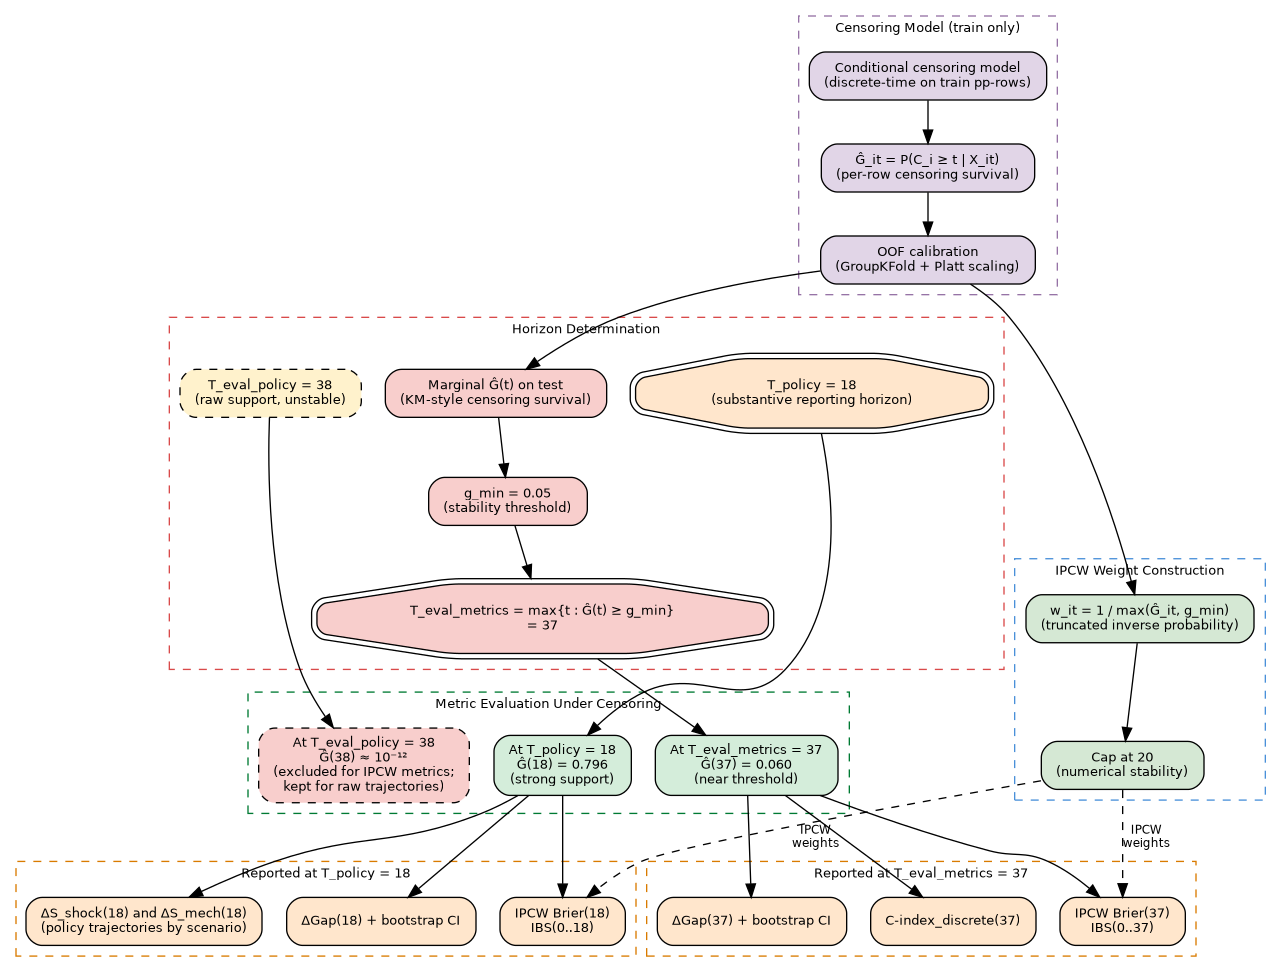
\includegraphics[width=\columnwidth]{figures/fig_censoring_dual_horizons.png}
\caption{Censoring-aware evaluation flow: the conditional censoring model determines IPCW weights and horizon stability, separating $T_{eval\_metrics}=37$ for weighted metrics from $T_{eval\_policy}=38$ for raw policy trajectories, with $T_{policy}=18$ as the substantive reporting horizon.}
\label{fig:censoring_dual_horizons}
\end{figure}

\paragraph*{Policy reporting horizon.}
$T_{policy}=18$ is the substantive horizon at which aggregate $\Delta S$ and subgroup $\Delta Gap$ are primarily reported. At this horizon, censoring survival is $\hat G(18)=0.796$, indicating strong support for IPCW-based summaries.

\paragraph*{Technical metric horizon.}
The stable IPCW horizon is
\begin{equation*}
T_{eval\_metrics}=\max\{t:\hat G(t)\ge g_{min}\},
\end{equation*}
with $g_{min}=0.05$, yielding $T_{eval\_metrics}=37$ and $\hat G(37)=0.060$. Beyond this point, $\hat G(38)\approx 10^{-12}$, making IPCW-based summaries numerically unstable. This horizon is therefore used as the last reliable point for weighted metric reporting.

\paragraph*{Raw support horizon.}
$T_{eval\_policy}=38$ denotes the maximum observed test support. It is retained for trajectory visualization only and is explicitly excluded from quantitative IPCW-based reporting.

\paragraph*{Censoring model.}
A conditional discrete-time model is fit on training person-period rows to estimate $\hat G_{it}=P(C_i\ge t \mid X_{it})$. Stabilized IPCW weights are defined as
\[
w_{it}=1/\max(\hat G_{it},\,g_{min}),
\]
and capped at 20 for numerical stability. Out-of-fold calibration is performed via GroupKFold plus Platt scaling. Together, these choices define the technical support conditions under which weighted metrics are reported.

%% -----------------------------------------------------------------------
\subsection{Primary and Secondary Metrics}
\label{subsec:metrics}

The metric suite is designed to distinguish discrimination, calibration, and horizon-specific predictive quality. Table~\ref{tab:metric_suite} maps each metric to the question it addresses and the horizon at which it is reported.

\begin{table}[!t]
\centering
\footnotesize
\renewcommand{\arraystretch}{1.05}
\caption{Evaluation metric suite and reporting horizons.}
\label{tab:metric_suite}
\begin{tabular}{@{}p{0.26\columnwidth} p{0.32\columnwidth} p{0.30\columnwidth}@{}}
\hline
Metric & Question addressed & Horizon(s) \\
\hline
$AUC_{row}$ &
  Row-level hazard discrimination &
  Full test support \\
IPCW Brier$(T)$ &
  Calibration at horizon $T$ &
  $T_{policy}$, $T_{eval}$ \\
IBS$(0{:}T)$ &
  Integrated calibration up to $T$ &
  $T_{policy}$, $T_{eval}$ \\
C-index$_{discrete}(T)$ &
  Ranking of event-time pairs &
  $T_{policy}$, $T_{eval}$ \\
ECE (15 bins) &
  Binned calibration error &
  Full test support \\
\hline
\end{tabular}
\end{table}

\paragraph*{Row-level AUC.}
AUC is computed on person-period test rows using target $event_{it}$ and score $\hat h_{it}$. Because the evaluation unit is the person-period row, this metric diagnoses row-level hazard discrimination rather than static enrollment-level classification performance.

\paragraph*{IPCW Brier score.}
Event probability at horizon $T$ is $\hat p_i^{(T)}=1-\hat S_i(T)$, with horizon label
\[
Y_i^{(T)}=\mathbb{1}\{E_i=1,\;t_i^{\mathrm{event}}\le T\}.
\]
The censoring-weighted Brier score~\cite{Graf1999AssessmentSurvivalPrediction} is
\begin{equation*}
BS_{IPCW}(T)=\frac{1}{n}\sum_i w_i(T)\left(Y_i^{(T)}-\hat p_i^{(T)}\right)^2.
\end{equation*}
This quantity evaluates horizon-specific probabilistic accuracy under censoring-aware weighting.

\paragraph*{Integrated Brier Score (IBS).}
\begin{equation*}
IBS(0{:}T)=\frac{1}{T+1}\sum_{t=0}^{T}BS_{IPCW}(t).
\end{equation*}
IBS summarizes calibration quality over an interval rather than at a single horizon, making it useful for comparing models over a span of weeks rather than at one fixed time point.

%% -----------------------------------------------------------------------
\subsection{Policy Evaluation Protocol (RQ2)}
\label{subsec:policy_eval}

The policy track compares two simulated regime constructions under the same deterministic trigger. This keeps the intervention rule fixed while isolating differences in how the regime is propagated through the model.

\paragraph*{Scenario specification.}
Table~\ref{tab:policy_spec} records the operational intervention anchor, and Table~\ref{tab:policy_intensity} records scenario-intensity assumptions. This separation makes explicit what is externally anchored versus what is treated as a simulation hypothesis.

\begin{table}[!t]
\centering
\caption{Operational intervention anchor (RQ2).}
\label{tab:policy_spec}
\begin{tabular}{lr}
\hline
Parameter & Value \\
\hline
$r^*$ (weekly proxy for 7-day inactivity) & 1 \\
Trigger frequency & weekly \\
$W$ (active window length) & 2 \\
Intervention class & short-term digital nudge \\
Anchor source & Kay \& Bostock (2023) \\
\hline
\end{tabular}
\end{table}

\begin{table}[!t]
\centering
\caption{Scenario-intensity assumptions for shock and shared mechanism-aware schedule (RQ2).}
\label{tab:policy_intensity}
\begin{tabular}{llp{0.53\columnwidth}}
\hline
Component & Value(s) & Interpretation \\
\hline
$\delta_{shock}$ & 0.08 & anchored conservative (qualitative anchor: Sneyers \& De Witte \cite{SneyersDeWitte2018InterventionsMeta}) \\
$\delta_{shock}$ & 0.20 & hypothetical A (legacy baseline) \\
$\delta_{shock}$ & 0.60 & hypothetical B (stress test) \\
$\alpha_{week0}$ & 0.35 & shared mechanism-aware schedule parameter \\
$\alpha_{week1}$ & 0.10 & shared mechanism-aware schedule parameter \\
Decay type & kb2023\_step\_2w & shared mechanism-aware schedule parameter \\
Window upper bound & exclusive & shared mechanism-aware schedule parameter \\
\hline
\end{tabular}
\end{table}

Operationally, the trigger and intervention class are anchored to Kay and Bostock \cite{KayBostock2023PowerNudge}, while shock intensity is treated as a scenario hypothesis under observational non-identification. The conservative scenario ($\delta_{shock}=0.08$) is anchored qualitatively, and the higher intensities are explicit hypothetical stress settings.

\paragraph*{Regimes compared.}
\begin{enumerate}
\item \textbf{Baseline regime ($a=0$):}
observed hazard trajectory $\hat h_{it}^{(0)}$.

\item \textbf{Shock regime ($a=1$, shock):}
hazard scaled by $(1-\delta_{shock,s})$ within active weeks, where $s$ indexes the scenario catalog.

\item \textbf{Mechanism-aware regime ($a=1$, mech):}
covariates overwritten within active weeks (click-based engagement boosted by schedule factor, activity/recency/streak propagated statefully), then hazard recomputed via plug-in prediction. The click perturbation is an LMS proxy analogous to participation/re-engagement dynamics in Kay and Bostock (2023), not a literal variable-level replication.
\end{enumerate}

Event rows are forced inactive in all regimes to prevent post-event counterfactual contamination. This rule ensures that counterfactual propagation only affects weeks in which the enrollment remains under risk.

\paragraph*{Outputs reported.}
For each regime, survival is reconstructed via the discrete-time product, and the aggregate structural contrast is
\[
\Delta S(t)=\bar S^{(1)}(t)-\bar S^{(0)}(t).
\]
Primary reporting for policy trajectories focuses on $\Delta S(T_{policy})$ and $\Delta S(T_{eval\_policy})$ by scenario; censoring-weighted metric diagnostics remain tied to $T_{eval\_metrics}$. These outputs provide the central empirical evidence for RQ2 under the interpretive contract of simulated regime comparison.

%% -----------------------------------------------------------------------
\subsection{Subgroup Evaluation Protocol (RQ3)}
\label{subsec:fairness_eval}

This track evaluates whether the same policy produces a differential change in outcome trajectories across observable groups, while preserving the same modeling and simulation engine used in the aggregate analysis.

\paragraph*{Demonstration variable.}
The fairness track uses \texttt{gender} as an operational demonstration variable with $g(i)\in\{0,1\}$. The framework itself is group-agnostic: the same protocol can be applied to any observable subgroup definition available in the dataset.

\paragraph*{Evaluated quantities.}
Under each regime $a\in\{0,1\}$, the following quantities are computed:
\begin{itemize}
\item groupwise mean survival $\bar\mu_g^{(a)}(t)$;
\item regime-specific gap $Gap^{(a)}(t)=\bar\mu_1^{(a)}(t)-\bar\mu_0^{(a)}(t)$;
\item change-in-gap $\Delta Gap(t)=Gap^{(1)}(t)-Gap^{(0)}(t)$.
\end{itemize}
All quantities are reported at both $T_{policy}=18$ and $T_{eval\_metrics}=37$. This mirrors the dual-horizon logic used in the aggregate policy track.

\paragraph*{Uncertainty via bootstrap.}
A total of $B=500$ bootstrap resamples with seed 42 are used to construct $95\%$ confidence intervals for $\Delta Gap(T)$. The reading rule is:
if $0\notin CI_{95\%}(\Delta Gap(T))$, the direction of gap change is considered robust at horizon $T$. This criterion provides an uncertainty-aware interpretation rather than relying on point estimates alone.

\paragraph*{Predictive fairness diagnostics.}
By-group row-level metrics (AUC, Brier, and ECE with 15 bins) and calibration curves are reported on test rows. Their role is to verify that subgroup-level policy contrasts are not being interpreted on top of severely asymmetric predictive quality across groups.

%% -----------------------------------------------------------------------
\subsection{Planned Robustness Battery}
\label{subsec:robustness}

The robustness plan was defined before examining comparative outcomes. Its purpose is to probe whether the main conclusions are sensitive to feature dependence, domain shift, or endpoint specification (Figure~\ref{fig:benchmark_robustness}).

% Placeholder for Graphviz figure (G4 benchmark_robustness)
% To produce: dot -Tpng graphviz_benchmark_robustness.txt -o figures/fig_benchmark_robustness.png
\begin{figure}[!t]
\centering
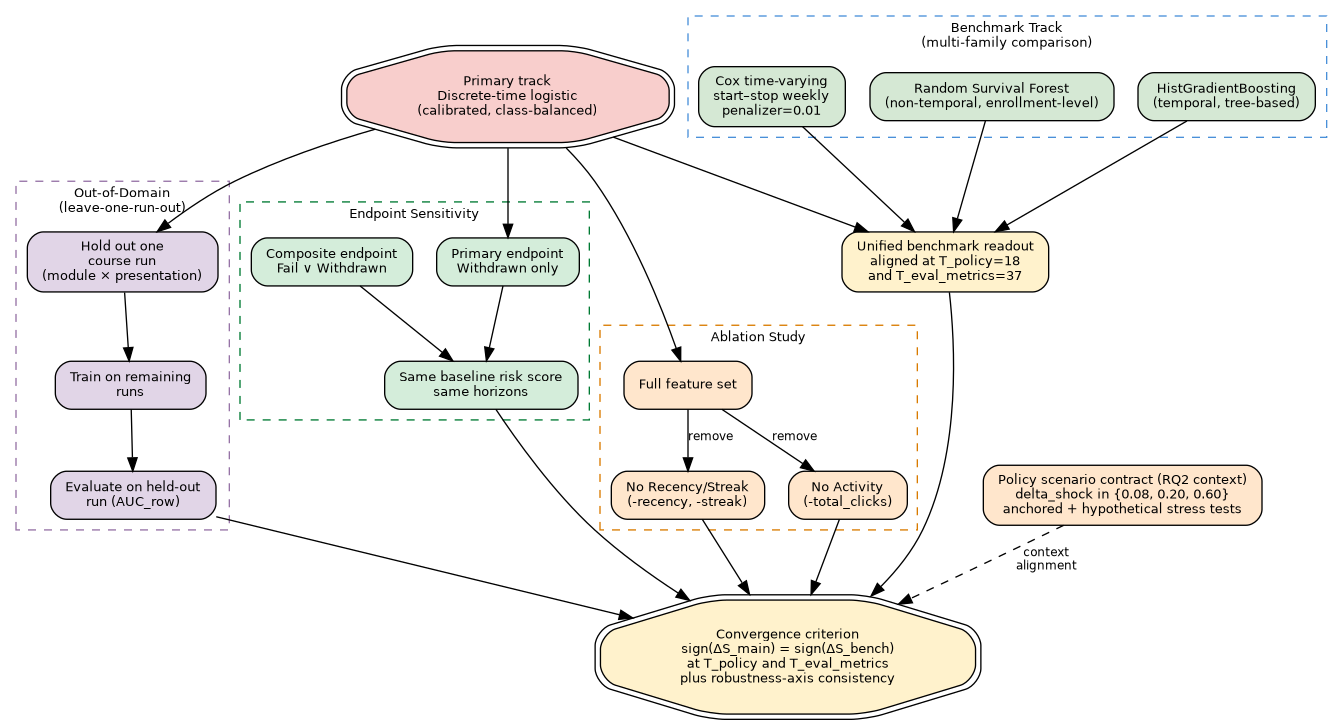
\includegraphics[width=\columnwidth]{figures/fig_benchmark_robustness.png}
\caption{Benchmark and robustness battery: the primary model is compared against alternative families (benchmark), feature subsets (ablation), unseen course runs (OOD), and an alternative endpoint (sensitivity), with convergence read at $T_{policy}$ and $T_{eval\_metrics}$ and interpreted under the scenario-aware RQ2 policy contract.}
\label{fig:benchmark_robustness}
\end{figure}

\paragraph*{Ablation study.}
Three model variants are retrained under the same protocol:
\begin{enumerate}
\item \textbf{Full:} all features;
\item \textbf{No Recency/Streak:} drops \texttt{recency} and \texttt{streak};
\item \textbf{No Activity:} drops \texttt{total\_clicks}.
\end{enumerate}
Each variant is retrained with
\texttt{LogisticRegression} with \texttt{solver="liblinear"},
\texttt{max\_iter=2000}, \texttt{class\_weight="balanced"}, and
\texttt{random\_state=42}
plus the same Platt calibration protocol. The leakage guard excludes all outcome and post-outcome fields. Metrics reported are $AUC_{row,test}$, $C\text{-index}_{discrete}(T_{eval})$, $BS_{IPCW}(T_{eval})$, and $IBS(0{:}T_{eval})$. This axis tests how dependent the main conclusions are on the core temporal engagement features.

\paragraph*{Out-of-domain generalization (leave-one-run-out).}
One entire course run $(\texttt{code\_module},\texttt{code\_presentation})$ is held out from training and used as the sole test set. The model is retrained on the remaining runs and evaluated via $AUC_{row}$ on the held-out person-period rows. Five held-out runs are reported to expose course-run heterogeneity and assess how far the main hazard model generalizes beyond pooled training conditions.

\paragraph*{Endpoint sensitivity.}
The primary endpoint is Withdrawn with valid unregistration date. As a sensitivity check, a composite endpoint (\textit{Fail} $\lor$ \textit{Withdrawn}) is evaluated using the \emph{same baseline risk score} $1-\hat S(t)$ produced by the model trained on the primary endpoint. For Fail cases, which lack an administrative unregistration date in OULAD, a terminal-time proxy based on the final observed week is used. Metrics are compared at the same horizons ($T_{policy}$, $T_{eval\_metrics}$). This sensitivity analysis tests whether the reading of results is materially altered by a broader operational endpoint.

%% -----------------------------------------------------------------------
\subsection{Comparison Rules and Reading Criteria}
\label{subsec:reading_criteria}

This subsection states explicitly how competing empirical signals are read. Its role is to prevent post hoc interpretation drift by fixing the directional rules used in comparative analysis.

\paragraph*{Sign consistency across families.}
The primary convergence check requires that the direction of $\Delta S$ be consistent between the main model and benchmarks:
\begin{equation*}
\mathrm{sign}\!\left(\Delta S_{main}(T)\right)
= \mathrm{sign}\!\left(\Delta S_{benchmark}(T)\right).
\end{equation*}
This rule does not require identical magnitudes across families; it requires agreement in the directional conclusion.

\paragraph*{Sign consistency in fairness.}
A fairness signal is considered robust when
\begin{equation*}
0 \notin CI_{95\%}\!\left(\Delta Gap(T)\right).
\end{equation*}
This criterion translates bootstrap uncertainty into a binary robustness reading for subgroup gap change at the reporting horizon.

\paragraph*{Stability across robustness axes.}
For each robustness axis $r$ (ablation, OOD, endpoint), robustness is assessed by directional stability:
\begin{equation*}
\mathrm{sign}\!\left(\Delta S_r(T)\right)
= \mathrm{sign}\!\left(\Delta S_{main}(T)\right),
\end{equation*}
while the spread within each axis is used as a sensitivity diagnostic. In this way, robustness is defined as preservation of the substantive conclusion under controlled design perturbations.

%% -----------------------------------------------------------------------
\subsection{Evidence Contract and Artifact Traceability}
\label{subsec:artifacts}

This subsection defines how empirical claims are tied to concrete outputs. It establishes the section's evidence contract and makes explicit the traceability expectations that later govern the Results section.

\paragraph*{Claim-to-evidence mapping.}
Every claim in Results must satisfy
\begin{equation*}
claim_j \;\rightarrow\; \{metric_j,\; figure_k,\; table_m,\; horizon_h\},
\end{equation*}
where figures and tables correspond to exported artifacts under \texttt{outputs\_v2/figures/} and \texttt{outputs\_v2/tables/}. This rule ensures that every interpretive statement can be audited back to a specific metric, artifact, and reporting horizon.

\paragraph*{Main text vs.\ appendix.}
The main text includes only evidence essential to the central argument, namely calibration, $\Delta S$, $\Delta Gap$, and benchmark convergence. Extended diagnostics, including per-group calibration curves, covariate delta profiles, and bootstrap histograms, are placed in the appendix. This separation keeps the main narrative focused while preserving auditability.

\paragraph*{Reproducibility.}
The complete pipeline---preprocessing, split generation, training and calibration, policy simulation, fairness diagnostics, and artifact export---is available at
\url{https://github.com/rafa-rodriguess/TCM-Student-Dropout}
\cite{RafaRepoTCMStudentDropout}. Horizon parameters ($T_{policy}$, $T_{eval\_policy}$, $T_{eval\_metrics}$, $g_{min}$), policy specification ($r^*$, $W$, shared mechanism-aware schedule, and scenario-indexed $\delta_{shock}$), and random seeds are recorded in the pipeline source. The scenario contract is exported in \nolinkurl{table_policy_scenarios_main.csv} and \nolinkurl{table_policy_scenario_params.csv}, with trajectory outputs exported in \nolinkurl{table_policy_deltaS_by_week_by_scenario.csv} and \nolinkurl{table_policy_deltaS_at_horizons_by_scenario.csv}. This traceability layer links the formal protocol described here to the executable notebook and exported evidence package.

%% -----------------------------------------------------------------------
\subsection{Executable Pipeline Summary}

Algorithm~\ref{alg:pipeline} summarizes the end-to-end executable pipeline from data integration through fairness evaluation. Its purpose is not to introduce new methodology, but to condense the protocol into a single operational sequence consistent with the previous subsections.

\begin{algorithm}[!t]
\caption{Discrete-Time Survival + Counterfactual Policy Simulation}
\label{alg:pipeline}
\small
\begin{algorithmic}[1]
\Require OULAD tables: \texttt{studentInfo}, \texttt{studentRegistration}, \texttt{studentVle}
\Ensure $\hat S^{(0)}(t)$, $\hat S^{(1)}(t)$, $\Delta S(T_{policy})$, $\Delta Gap(T)$ with bootstrap CI, exported artifacts

\State Build enrollment backbone keyed by $(\texttt{id\_student},\texttt{code\_module},\texttt{code\_presentation})$.
\State Define endpoint: $E_i=\mathbb{1}[\texttt{Withdrawn} \wedge \texttt{date\_unregistration valid}]$; $t^{event}_i=\lfloor \texttt{date\_unregistration}/7 \rfloor$.
\State Compute censoring anchor $t^{last}_i$ (last observed week with non-negative VLE activity; default 0).
\State Define $t^{final}_i$: $t^{event}_i$ if $E_i=1$; $t^{last}_i$ otherwise.
\State Construct weekly person-period rows $t=0,\dots,t^{final}_i$ with $event_{it}=\mathbb{1}[E_i=1 \wedge t=t^{final}_i]$.
\State Engineer weekly covariates $X_{it}$ (clicks, Recency, Streak, submitted) using $w(d)=\max(\lfloor d/7\rfloor,0)$.
\State Perform enrollment-stratified temporal split with $q=4$ buckets and \texttt{test\_size}=0.30.
\State Fit the discrete-time hazard model on training rows (penalized, class-balanced logistic + sigmoid calibration).
\State Compute $\hat h^{(0)}_{it}$ on test rows; reconstruct $\hat S^{(0)}_i(t)=\prod_{k\le t}(1-\hat h^{(0)}_{ik})$.
\State Apply the Recency-triggered policy ($r^*=1$, $W=2$) under scenario catalog $\delta_{shock}\in\{0.08,0.20,0.60\}$:
\State \hspace{6pt} \textit{Shock:} $\hat h^{(1,shock,s)}_{it}=\hat h^{(0)}_{it}(1-\delta_{shock,s})$ when active.
\State \hspace{6pt} \textit{Mechanism-aware:} overwrite covariates in the active window (primarily click-based engagement), propagate statefully, and recompute $\hat h^{(1,mech)}_{it}=f(X^{cf}_{it})$.
\State Compute $\hat S^{(1)}_i(t)$ for each regime and scenario; report $\Delta S(T_{policy})$ and $\Delta S(T_{eval\_policy})$ by scenario.
\State Report diagnostics: $AUC_{row}$, $BS_{IPCW}$, and IBS at both horizons.
\State Perform subgroup validation (RQ3): compute $\bar\mu^{(a)}_g(t)$, $Gap^{(a)}(t)$, and $\Delta Gap(t)$ at $T_{policy}=18$ and $T_{eval}=37$.
\State \hspace{6pt} Summarize subgroup uncertainty using $B=500$ bootstrap confidence intervals.
\end{algorithmic}
\end{algorithm}

%% -----------------------------------------------------------------------
\subsection{Limits of the Experimental Design}
\label{subsec:design_limits}

The experimental design evaluates temporal predictive quality and structural regime contrasts under explicit protocol rules; it does not constitute a causal identification design for intervention effects. These limits are part of the section's interpretive contract and should be read together with the evidence rules defined above.

Specifically:
\begin{itemize}
\item Policy and fairness results are \textit{model-implied simulated regime contrasts} under fixed scenario parameters, not observationally identified effects.
\item The censoring treatment uses IPCW for evaluation diagnostics, but it does not apply censoring-weighted retraining or pursue causal identification strategies for potentially informative censoring.
\item Out-of-domain generalization is evaluated via leave-one-run-out, but the pooled training strategy does not explicitly model instructional heterogeneity across course runs.
\item The endpoint sensitivity analysis does not impute event times for Fail cases; instead, it uses a terminal-time proxy based on the final observed week because OULAD does not provide an administrative withdrawal timestamp for Fail.
\end{itemize}

These boundaries define what the reader should and should not infer from the results. The section promises a transparent, pre-specified, and executable evaluation design for temporal prediction, regime comparison, and subgroup diagnostics; it does not promise causal effect estimation from observational exposure.
\section{Results}

This section reports the empirical evidence generated by the executable pipeline and answers the three research questions directly. Its purpose is not only to present metric values, but also to show how the evidence should be read under the protocol defined in Methodology and Experimental Design. Throughout the section, the interpretation contract is preserved: policy and fairness quantities are reported as \textit{model-implied simulated regime contrasts}, not as observationally identified intervention effects.

The section follows the same logical progression as the framework itself. It begins with a figure-reading guide and direct answers to the research questions, then presents evidence for RQ1 (hazard quality), establishes the censoring-valid horizons required for interpreting downstream results, reports policy contrasts for RQ2, examines benchmark and robustness evidence, and finally reports subgroup results for RQ3. By the end of the section, the reader should expect a complete empirical answer to the paper objective: whether the framework can translate weekly risk into auditable policy and subgroup diagnostics under explicit reporting rules.

\subsection{How to Read the Figures in This Section}

To avoid ambiguous interpretation, each figure is tied to one research question, one metric family, and one reading rule. Table~\ref{tab:fig_reading_guide} summarizes that mapping and should be read as the figure-level evidence contract for this section.

\begin{table}[!t]
\centering
\scriptsize
\renewcommand{\arraystretch}{1.05}
\caption{Figure reading guide used in Results.}
\label{tab:fig_reading_guide}
\begin{tabular}{@{}>{\raggedright\arraybackslash}p{0.24\columnwidth}
                >{\raggedright\arraybackslash}p{0.24\columnwidth}
                >{\raggedright\arraybackslash}p{0.42\columnwidth}@{}}
\hline
Figure & What it answers & How to read it \\
\hline
Calibration reliability test &
RQ1 hazard quality &
Curves close to the diagonal indicate calibrated weekly risk. \\

Policy survival by week &
Temporal risk window (RQ1--RQ2 bridge) &
Compare slopes and separation near $T_{policy}$, $T_{eval\_metrics}$, and raw-support tail $T_{eval\_policy}$. \\

Censoring survival $G(t)$ &
Horizon validity under censoring &
Identify where $G(t)$ drops below $g_{min}=0.05$. \\

Policy $\Delta S(t)$ by week &
RQ2 policy contrast &
Positive $\Delta S(t)$ means policy survival exceeds baseline survival. \\

Benchmark dual-panel AUC &
Family robustness &
Check directional consistency across model families. \\

RQ3 gap at $T_{policy}$ and $T_{eval\_metrics}$ &
RQ3 subgroup contrast &
Read the sign and uncertainty of $\Delta Gap(T)$ at $T_{policy}$ and $T_{eval\_metrics}$. \\
\hline
\end{tabular}
\end{table}

\subsection{Direct Answers to the Research Questions}
\label{subsec:direct_answers}

Table~\ref{tab:rq_answers} gives the direct empirical answers before the detailed evidence is unpacked. The remainder of the section then substantiates each answer with figures, tables, and horizon-specific interpretation rules.

\begin{table}[!t]
\centering
\scriptsize
\renewcommand{\arraystretch}{1.05}
\caption{Direct answers to RQ1--RQ3 at reported horizons.}
\label{tab:rq_answers}
\begin{tabular}{@{}>{\raggedright\arraybackslash}p{0.12\columnwidth}
                >{\raggedright\arraybackslash}p{0.82\columnwidth}@{}}
\hline
RQ & Direct answer from results \\
\hline
RQ1 &
Yes. Weekly hazard discrimination is stable (AUC train 0.8350, test 0.8405), and calibration diagnostics support the use of hazard trajectories for decision timing. \\

RQ2 &
Yes, with strong scenario dependence under a fixed trigger. At $T_{policy}=18$, shock contrasts are $\Delta S=0.0102$ (anchored conservative, $\delta=0.08$), $0.0260$ (hypothetical A, $\delta=0.20$), and $0.0819$ (hypothetical B, $\delta=0.60$), while the mechanism-aware contrast is $\Delta S=-0.0006$. \\

RQ3 &
Yes, in directional terms. $\Delta Gap(T_{policy})=-0.00050816$ and $\Delta Gap(T_{eval\_metrics})=-0.00056691$, with 95\% bootstrap intervals excluding zero at both horizons, indicating a robust direction under the reported scenario. \\
\hline
\end{tabular}
\end{table}

\subsection{RQ1: Temporal Hazard Quality and Actionable Timing}
\label{subsec:rq1_results}

RQ1 asks whether the temporal model is good enough to support downstream policy and subgroup evaluation. The empirical answer depends on two elements: weekly hazard discrimination and calibration quality over operationally relevant risk ranges.

\paragraph*{Discrimination.}
Under the enrollment-level stratified temporal split, row-level weekly hazard discrimination is
\begin{equation*}
AUC_{train}=0.8350, \qquad AUC_{test}=0.8405.
\end{equation*}
The small train--test gap indicates that performance remains stable under temporal holdout rather than collapsing out of sample. This supports the use of the fitted hazard model as the backbone for subsequent simulated-regime analysis.

\paragraph*{Calibration and weekly interpretation.}
Figure~\ref{fig:calibration_main} provides the primary calibration evidence for RQ1. It should be read as a reliability diagnostic for weekly hazard probabilities: if predicted risk bins and observed frequencies remain close, the hazard scale can be treated as sufficiently trustworthy for downstream regime simulation and decision timing.

\begin{figure}[!t]
\centering
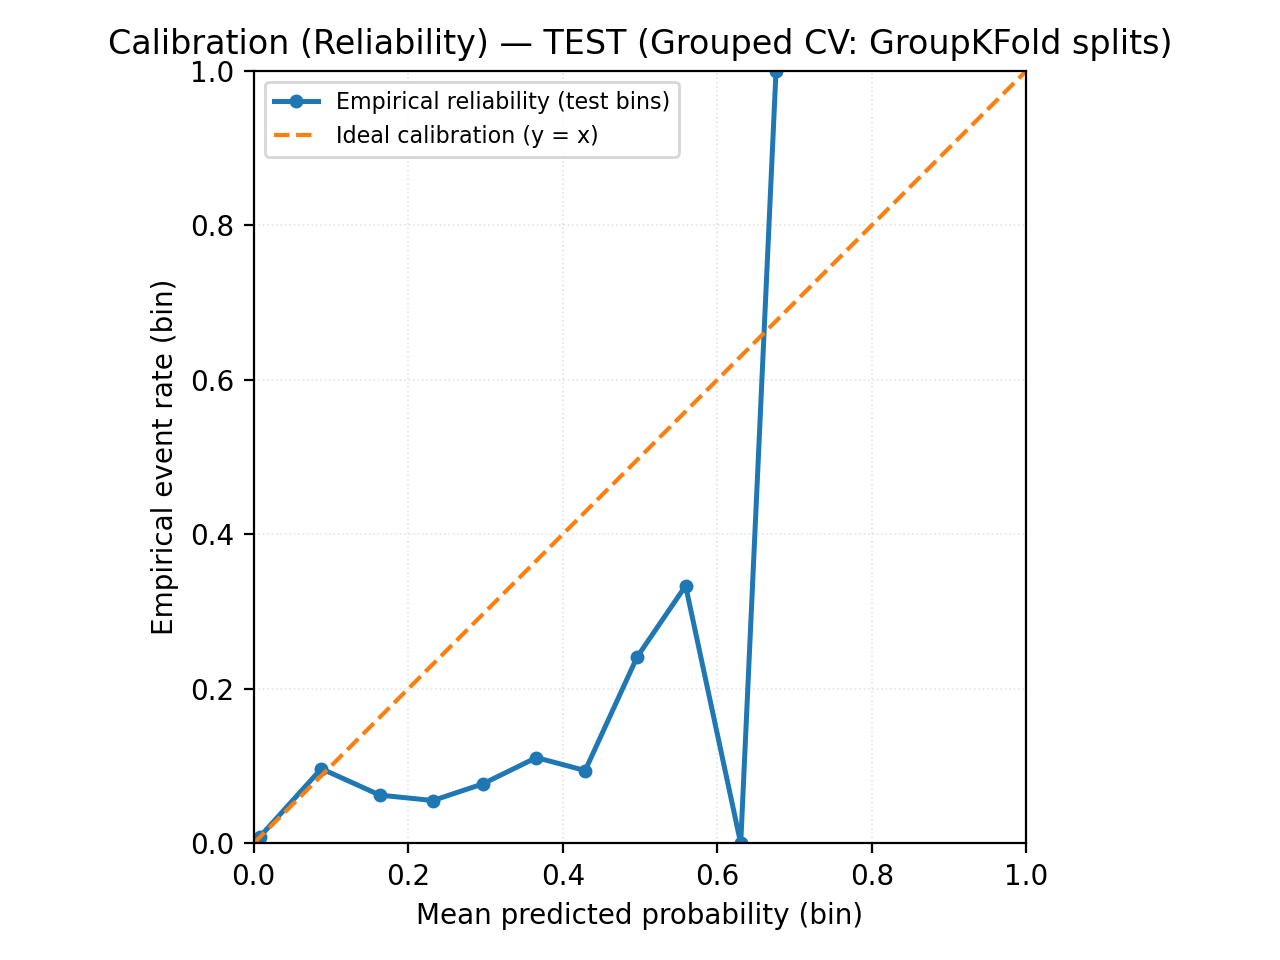
\includegraphics[width=0.45\textwidth]{outputs_v2/figures/fig_calibration_reliability_test.png}
\caption{Primary calibration evidence for weekly hazard on test rows. The figure supports the RQ1 claim only if reliability remains acceptable over operationally relevant risk bins.}
\label{fig:calibration_main}
\end{figure}

To make the right-tail reading fully auditable, Table~\ref{tab:calibration_tail_support} reports support for the highest-risk bins in the same partition used by Figure~\ref{fig:calibration_main}. The key readout is direct sample support ($n$, events, and non-events) for each tail bin.

\begin{table}[!t]
\centering
\caption{Support of the highest-risk calibration bins on test rows (same binning as Figure~\ref{fig:calibration_main}).}
\label{tab:calibration_tail_support}
\begin{tabular}{lcccc}
\hline
Bin & Risk interval & $n$ & Events & Non-events \\
\hline
Bin 8 & [0.533, 0.600) & 9 & 3 & 6 \\
Bin 9 & [0.600, 0.667) & 7 & 0 & 7 \\
Bin 10 & [0.667, 0.733) & 3 & 3 & 0 \\
\hline
\end{tabular}
\end{table}

\paragraph*{When to act: temporal decision window.}
Figure~\ref{fig:survival_baseline_rq1} connects predictive quality to decision timing. It places the baseline and policy trajectories on a common weekly axis with $T_{policy}=18$, $T_{eval\_metrics}=37$, and raw-support tail at $T_{eval\_policy}=38$. For RQ1, the baseline trajectory is the key object: periods of steeper decline define the weeks in which temporal monitoring is most decision-relevant.

\begin{figure}[!t]
\centering
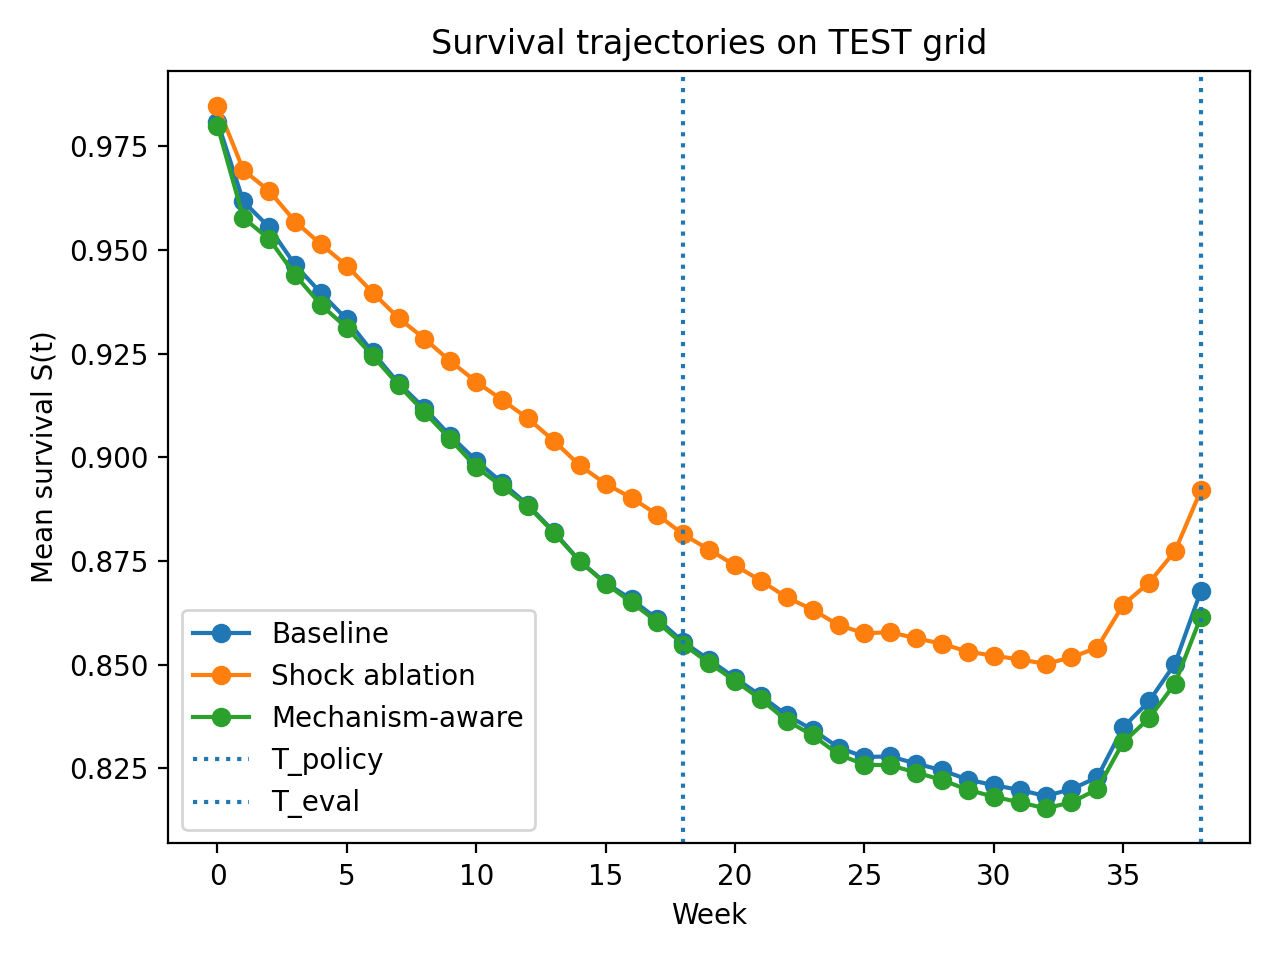
\includegraphics[width=0.45\textwidth]{outputs_v2/figures/fig_policy_survival_by_week_baseline_shock_mech.png}
\caption{Mean survival trajectories by week. For RQ1, the baseline curve is the key object: steeper decline windows indicate periods where temporal monitoring is most decision-relevant.}
\label{fig:survival_baseline_rq1}
\end{figure}

\paragraph*{RQ1 conclusion.}
Taken together, the discrimination and calibration evidence supports the intended use of the model: translating weekly risk into auditable timing signals. This conclusion, however, remains subject to the censoring-valid horizons established next.

\subsection{Censoring Validity and the Dual-Horizon Rule}
\label{subsec:censoring_results}

Before reading the RQ2 and RQ3 contrasts, the validity of the reporting horizons must be established. Figure~\ref{fig:censoring_survival_results} displays the estimated censoring survival $G(t)$ on the test set and provides the empirical justification for using two horizons rather than one.

\begin{figure}[!t]
\centering
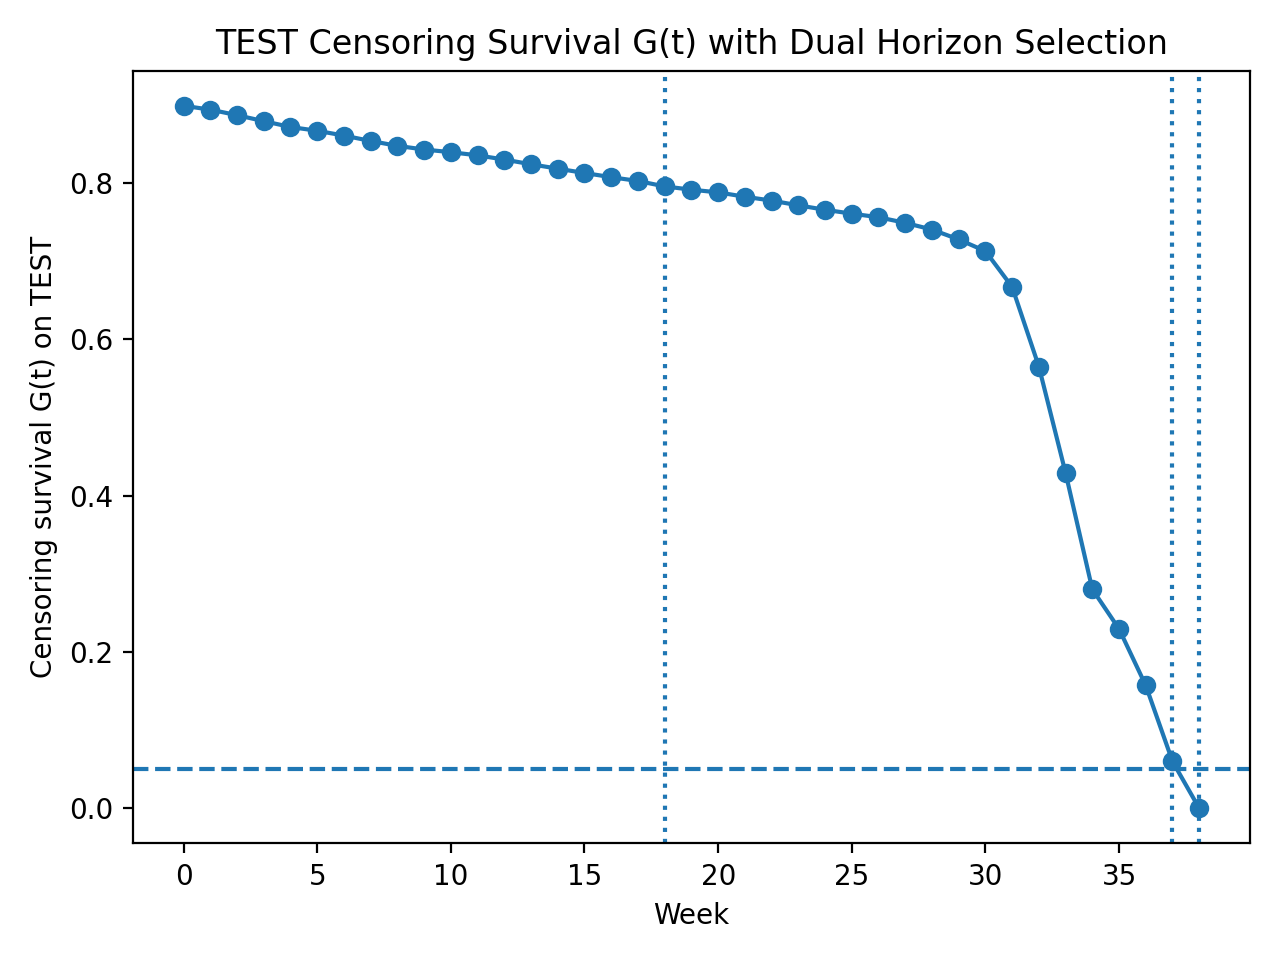
\includegraphics[width=0.45\textwidth]{outputs_v2/figures/fig_censoring_survival_G_test.png}
\caption{Censoring survival $G(t)$ used to define stable reporting horizons. The reading rule is operational: IPCW metrics are interpreted only where $G(t) \ge g_{min}=0.05$.}
\label{fig:censoring_survival_results}
\end{figure}

\begin{table}[!t]
\centering
\caption{Censoring-aware horizon diagnostics used in Results.}
\label{tab:horizon_diagnostics}
\begin{tabular}{lc}
\hline
Quantity & Value \\
\hline
$T_{policy}$ & 18 \\
$T_{eval\_metrics}$ (stable IPCW horizon) & 37 \\
$T_{eval\_policy}$ (raw support horizon) & 38 \\
$G(18)$ & 0.7958 \\
$G(37)$ & 0.0601 \\
$G(38)$ & $\approx 10^{-12}$ (unstable) \\
\hline
\end{tabular}
\end{table}

This rule is not cosmetic. It is part of the evidence contract of the section: weighted metrics and contrast summaries are interpreted only at horizons with acceptable censoring support. The distinction between $T_{policy}$, $T_{eval\_metrics}$, and $T_{eval\_policy}$ therefore determines where substantive claims are allowed to be made.

\subsection{RQ2: Policy Simulation and Structural Regime Contrast}
\label{subsec:rq2_results}

RQ2 asks whether an explicit policy rule changes model-implied survival trajectories under fixed protocol settings. The results show that the answer is yes, but the magnitude of the contrast depends strongly on how the policy enters the system.

\paragraph*{Definition used in reporting.}
\begin{equation*}
\Delta S(t)=\bar S^{(1)}(t)-\bar S^{(0)}(t),
\qquad
\bar S^{(a)}(t)=\frac{1}{N}\sum_i \hat S_i^{(a)}(t).
\end{equation*}
Positive $\Delta S(t)$ means higher survival under the policy regime than under baseline.

\paragraph*{Figure-level evidence for RQ2.}
Figure~\ref{fig:deltas_rq2} is the primary figure for RQ2. It should be read in two steps:
first, the sign over time (is the contrast above zero?);
second, the horizon-specific magnitude by scenario (what is $\Delta S$ at $T_{policy}$ and $T_{eval\_policy}$?).

\begin{figure}[!t]
\centering
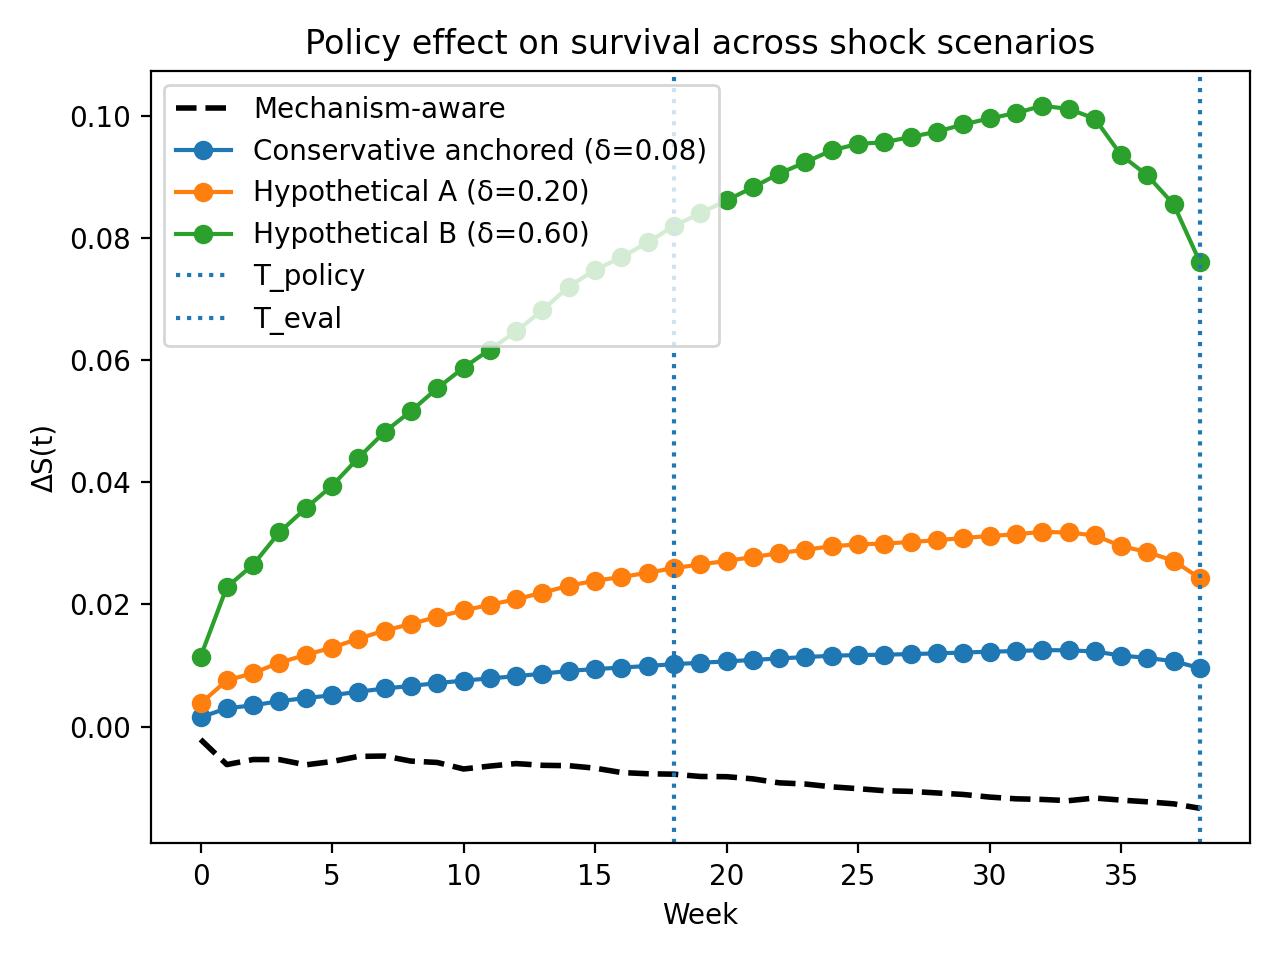
\includegraphics[width=0.45\textwidth]{outputs_v2/figures/fig_policy_deltaS_by_week_shock_scenarios.png}
\caption{Policy contrast $\Delta S(t)$ under a fixed trigger with scenario-indexed shock intensity ($\delta\in\{0.08,0.20,0.60\}$) and the shared mechanism-aware curve. The central readout is sign and horizon-specific magnitude by scenario.}
\label{fig:deltas_rq2}
\end{figure}

\begin{table}[!t]
\centering
\caption{RQ2 summary by shock-intensity scenario at $T_{policy}=18$ and $T_{eval\_policy}=38$.}
\label{tab:rq2_summary}
\small
\begin{tabular}{lcccc}
\hline
Scenario & $\delta_{shock}$ & $\Delta S_{shock}(18)$ & $\Delta S_{shock}(38)$ & $\Delta S_{mech}(18)$ \\
\hline
Anchored conservative & 0.08 & 0.0102 & 0.0096 & -0.0006 \\
Hypothetical A (reference) & 0.20 & 0.0260 & 0.0243 & -0.0006 \\
Hypothetical B (stress test) & 0.60 & 0.0819 & 0.0760 & -0.0006 \\
\hline
\end{tabular}
\end{table}

The shared mechanism-aware contrast is $\Delta S_{mech}(38)=-0.0062$ at $T_{eval\_policy}$, indicating that under the current schedule and propagated covariate channel, the mechanism-aware regime does not generate a positive survival gain in this run.

\paragraph*{Mechanism diagnostic.}
To explain why the shock and mechanism-aware regimes differ so sharply, Figure~\ref{fig:policy_mechanism_deltas} should be read as a transmission diagnostic. It shows whether policy-induced covariate deltas are large enough, and persistent enough, to alter downstream hazard meaningfully.

\begin{figure}[!t]
\centering
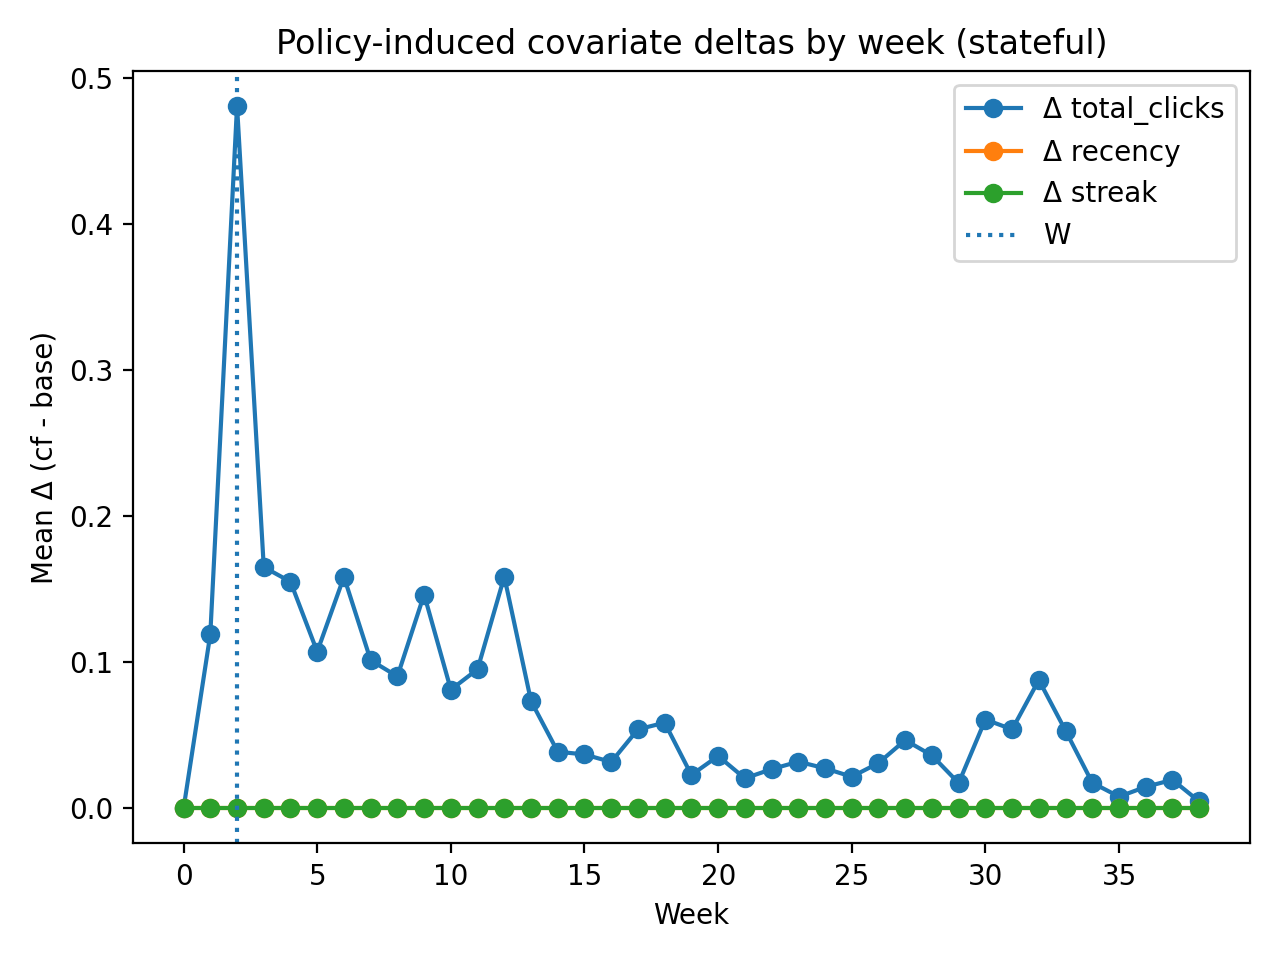
\includegraphics[width=0.45\textwidth]{outputs_v2/figures/fig_policy_covariate_deltas_by_week.png}
\caption{Mechanism diagnostic for policy propagation. Small or short-lived covariate deltas imply limited downstream hazard movement, consistent with the weak/negative mechanism-aware contrasts at fixed horizons in this run.}
\label{fig:policy_mechanism_deltas}
\end{figure}

\paragraph*{RQ2 conclusion.}
The framework answers RQ2 positively in structural terms: it can compare explicit regimes on a common temporal backbone and produce interpretable survival contrasts at fixed horizons. In the present configuration, the contrast is highly scenario-dependent in the shock branch (larger gains for larger $\delta$), while the mechanism-aware branch remains weak to negative under the current shared schedule.

\subsection{Benchmark and Robustness Evidence}
\label{subsec:benchmark_robust_results}

The purpose of this subsection is not to replace the primary track, but to test whether the main interpretation remains stable under benchmark comparison and controlled design perturbations. The benchmark families used here are the \textit{Cox time-varying benchmark} and the \textit{non-temporal enrollment-level benchmark}; together, they provide the main cross-family reference against which the primary discrete-time model is read.

\paragraph*{Cross-family benchmark.}
Figure~\ref{fig:benchmark_dual_panel} summarizes the primary model against benchmark families at aligned horizons. The key readout is directional convergence rather than rank ordering alone: the question is whether the substantive conclusion remains consistent across model families.

\begin{figure}[!t]
\centering
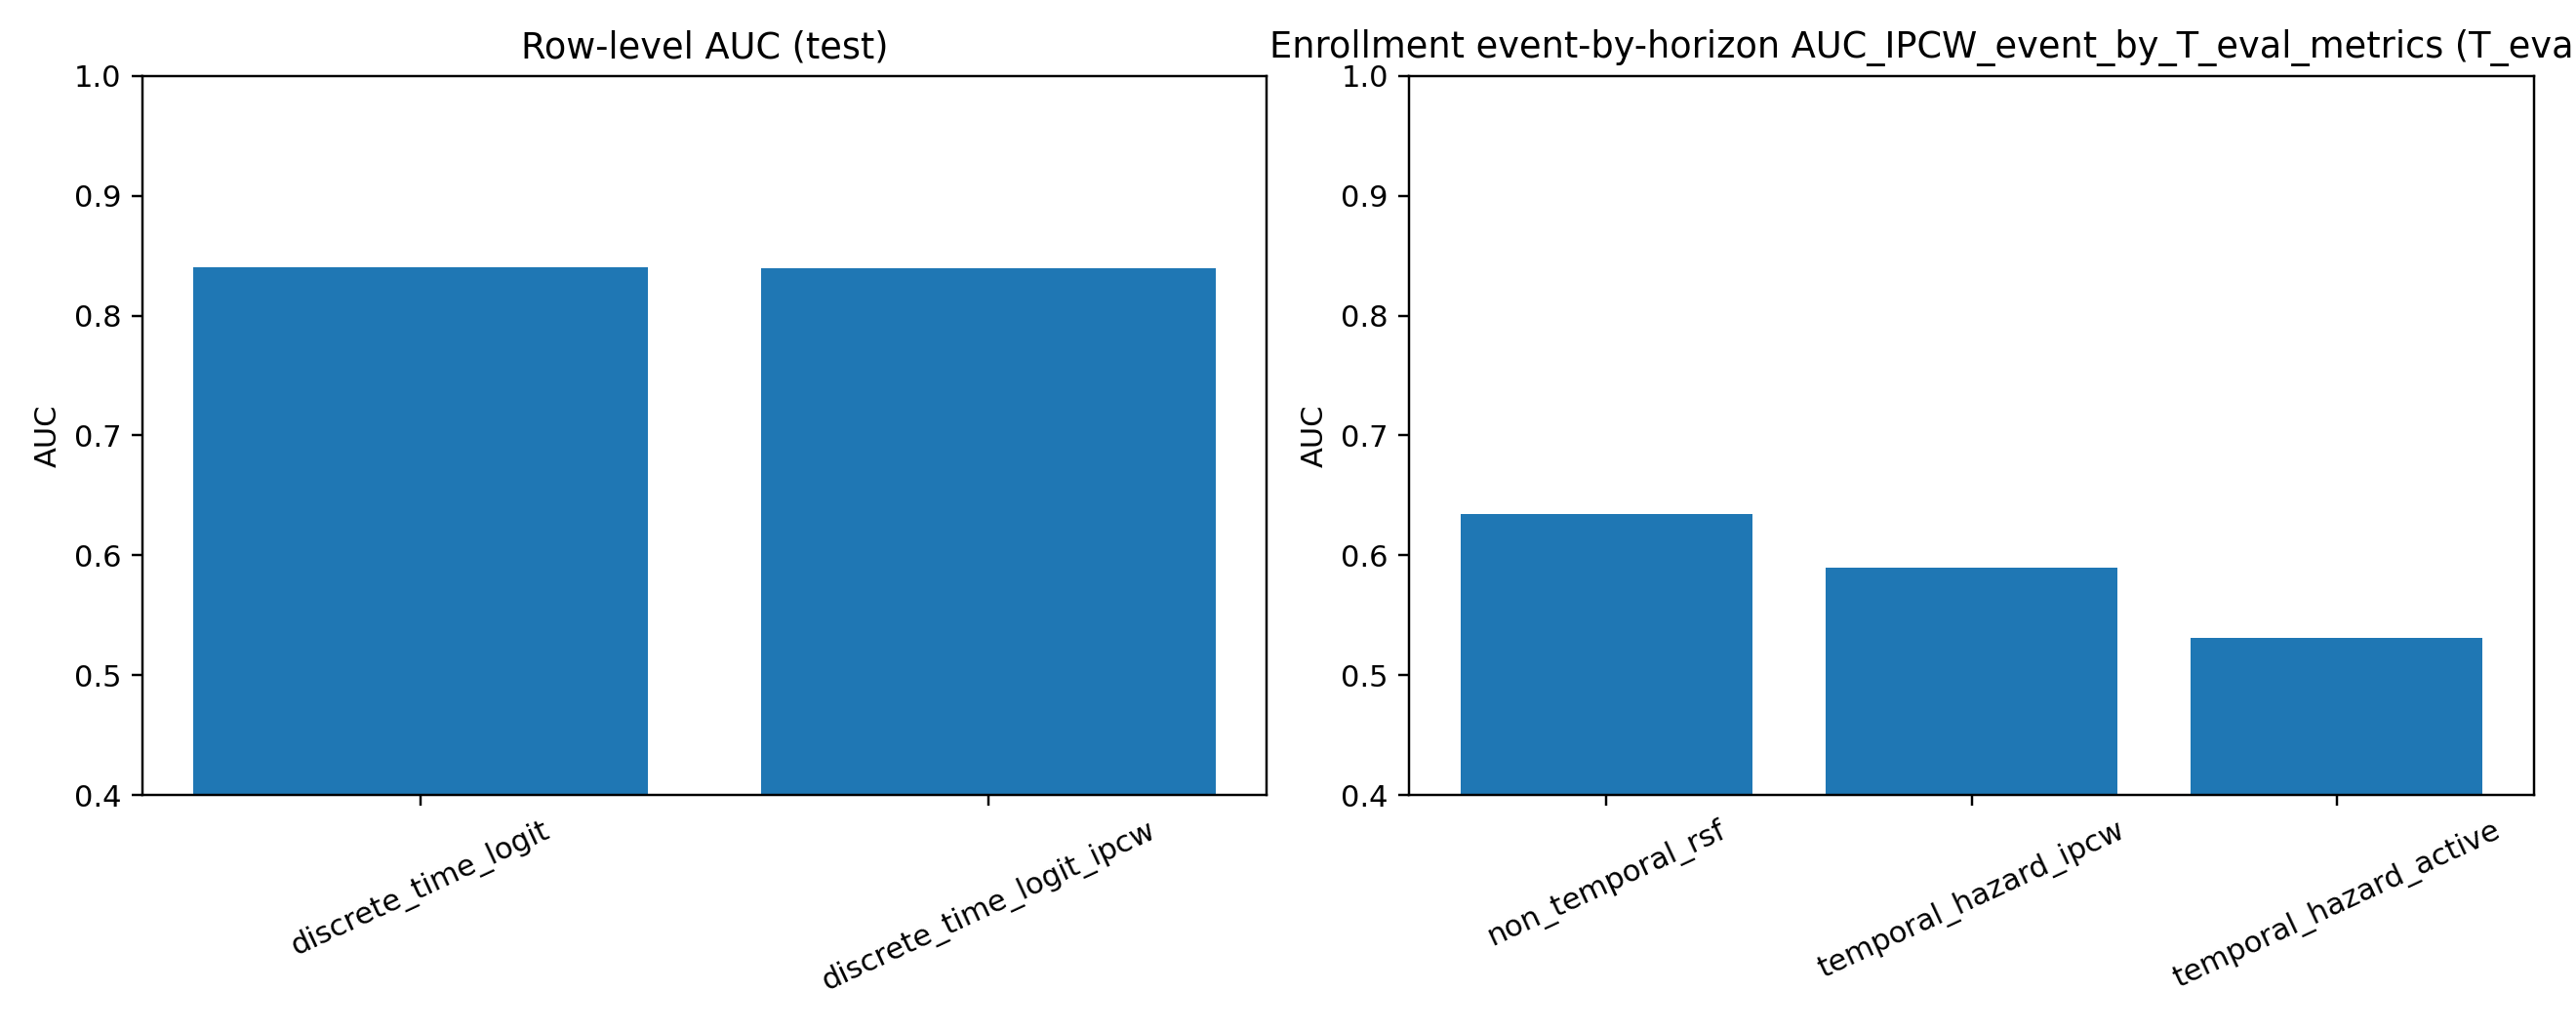
\includegraphics[width=0.45\textwidth]{outputs_v2/figures/fig_benchmark_dual_panel_auc.png}
\caption{Benchmark comparison across model families. Use this figure to verify whether the central directional conclusion is stable across the primary model, the Cox benchmark, and the non-temporal baseline.}
\label{fig:benchmark_dual_panel}
\end{figure}

\paragraph*{Ablation evidence.}
\begin{table}[!t]
\centering
\caption{Ablation at $T_{eval\_metrics}=37$ (re-trained variants).}
\label{tab:ablation_results}
\resizebox{\columnwidth}{!}{%
\begin{tabular}{lcccc}
\hline
Model & AUC$_{row,test}$ & C-index$_{discrete}$ & IPCW Brier & IPCW IBS \\
\hline
Full & 0.8396 & 0.3951 & 0.3392 & 0.1747 \\
No Recency/Streak & 0.7987 & 0.3637 & 0.3728 & 0.1772 \\
No Activity (\texttt{total\_clicks}) & 0.8263 & 0.3369 & 0.3530 & 0.1781 \\
\hline
\end{tabular}%
}
\end{table}

Removing Recency/Streak causes the largest AUC drop, which is consistent with the proposed role of temporal regularity features in supporting weekly hazard quality.

\paragraph*{Endpoint sensitivity.}
\begin{table}[!t]
\centering
\caption{Endpoint sensitivity at $T_{eval\_metrics}=37$.}
\label{tab:endpoint_sensitivity_results}
\resizebox{\columnwidth}{!}{%
\begin{tabular}{lcc}
\hline
Metric & Primary (Withdrawn) & Composite (Fail OR Withdrawn) \\
\hline
C-index$_{discrete}(T_{eval\_metrics})$ & 0.4965 & 0.4965 \\
IPCW Brier($T_{eval\_metrics}$) & 0.8542 & 1.0799 \\
IPCW IBS($0..T_{eval\_metrics}$) & 0.2429 & 0.3291 \\
$N_{events}$ & 2{,}216 & 4{,}308 \\
\hline
\end{tabular}%
}
\end{table}

The directional reading is preserved, while calibration and risk quality shift under endpoint broadening. This is the intended role of this robustness axis: to show where the conclusion is stable and where metric quality changes under alternative endpoint definitions.

\paragraph*{Out-of-domain generalization.}
\begin{table}[!t]
\centering
\caption{Held-out run generalization (five runs).}
\label{tab:ood_results_short}
\small
\resizebox{\columnwidth}{!}{%
\begin{tabular}{lrrrrr}
\hline
Held-out run & Rows & Pos. rate & AUC$_{row}$ & Enrollments & Events \\
\hline
\texttt{CCC-2014J} & 57{,}760 & 0.0145 & 0.7652 & 2{,}498 & 836 \\
\texttt{FFF-2014J} & 56{,}546 & 0.0112 & 0.8393 & 2{,}365 & 636 \\
\texttt{BBB-2014J} & 52{,}440 & 0.0095 & 0.7934 & 2{,}292 & 497 \\
\texttt{FFF-2013J} & 57{,}054 & 0.0088 & 0.8317 & 2{,}283 & 504 \\
\texttt{BBB-2013J} & 52{,}849 & 0.0078 & 0.8381 & 2{,}237 & 410 \\
\hline
\end{tabular}%
}
\end{table}

AUC variability across held-out runs reveals course-run heterogeneity. This limits direct portability across settings, but it does not invalidate the framework itself; rather, it identifies the scale at which domain sensitivity should be expected.

\subsection{RQ3: Subgroup Validation via Change-in-Gap}
\label{subsec:rq3_results}

RQ3 tests whether the same policy regime produces differential group contrasts, reported with uncertainty. The emphasis here is not on a broad fairness claim, but on whether the framework can quantify subgroup-sensitive structural contrasts on the same simulation backbone used for aggregate policy evaluation.

\paragraph*{Reported quantity.}
\begin{equation*}
\Delta Gap(T)=Gap^{(1)}(T)-Gap^{(0)}(T).
\end{equation*}
Negative values indicate reduced gap under policy relative to baseline for the group coding used in this run.

\paragraph*{Primary figure-level evidence.}
The fairness interpretation pipeline is summarized in Figure~\ref{fig:fairness_pipeline_graph}. Figures~\ref{fig:rq3_gap_tpolicy} and \ref{fig:rq3_gap_teval} are then read as horizon-specific outputs of that pipeline.

\begin{figure}[!t]
\centering
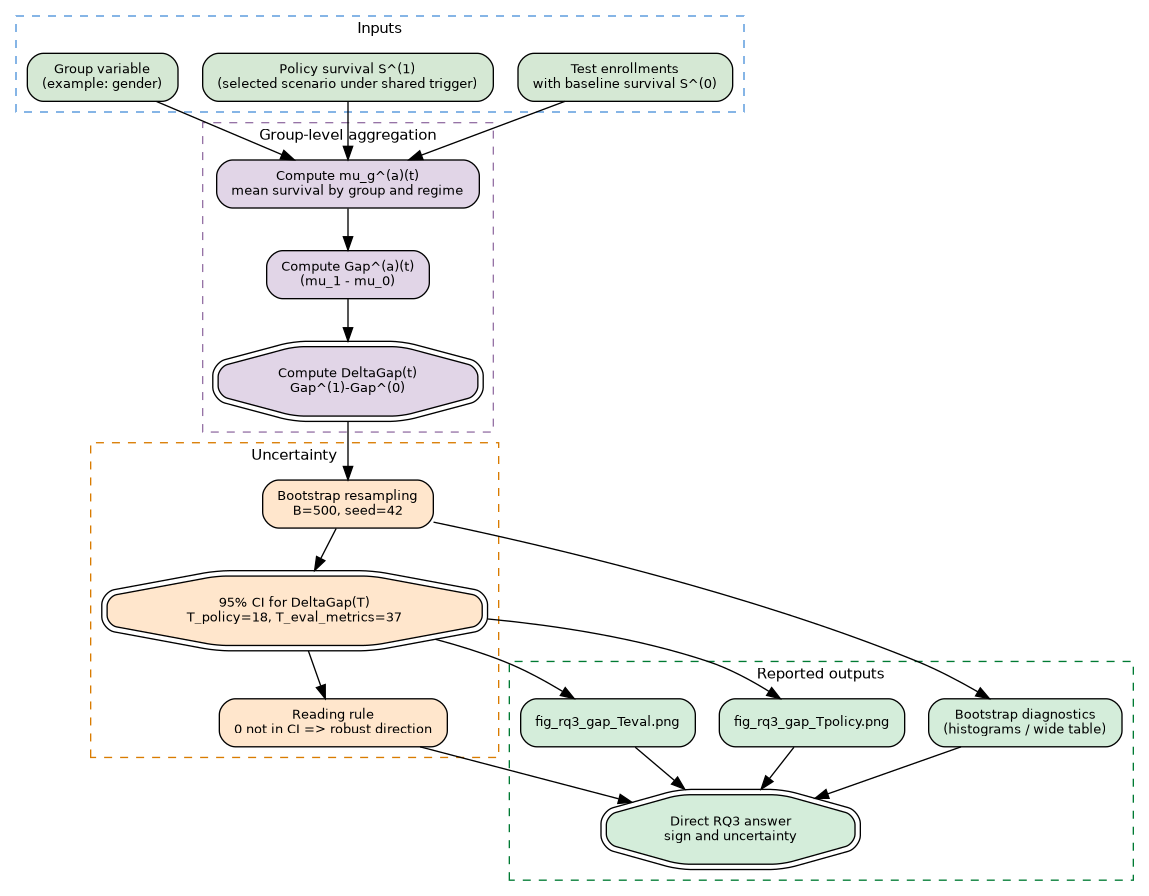
\includegraphics[width=0.45\textwidth]{figures/fig_fairness_pipeline.png}
\caption{Fairness/subgroup pipeline used in RQ3. It links groupwise survival aggregation, change-in-gap computation, and bootstrap uncertainty for a selected policy scenario under the shared trigger contract.}
\label{fig:fairness_pipeline_graph}
\end{figure}

\begin{figure}[!t]
\centering
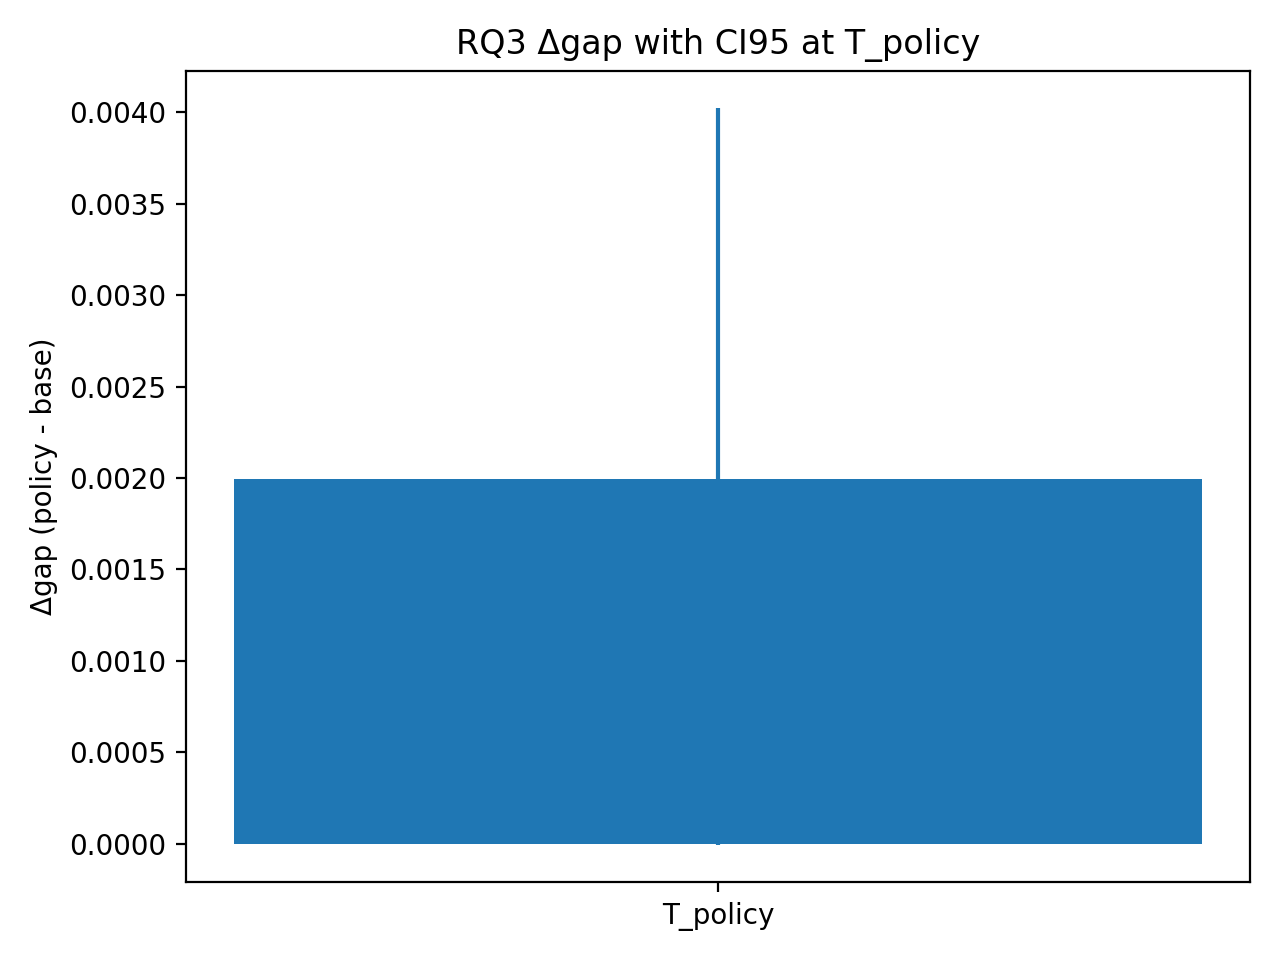
\includegraphics[width=0.45\textwidth]{outputs_v2/figures/fig_rq3_gap_Tpolicy.png}
\caption{RQ3 gap result at $T_{policy}=18$. Interpretation requires combining sign, magnitude, and confidence-interval support.}
\label{fig:rq3_gap_tpolicy}
\end{figure}

\begin{figure}[!t]
\centering
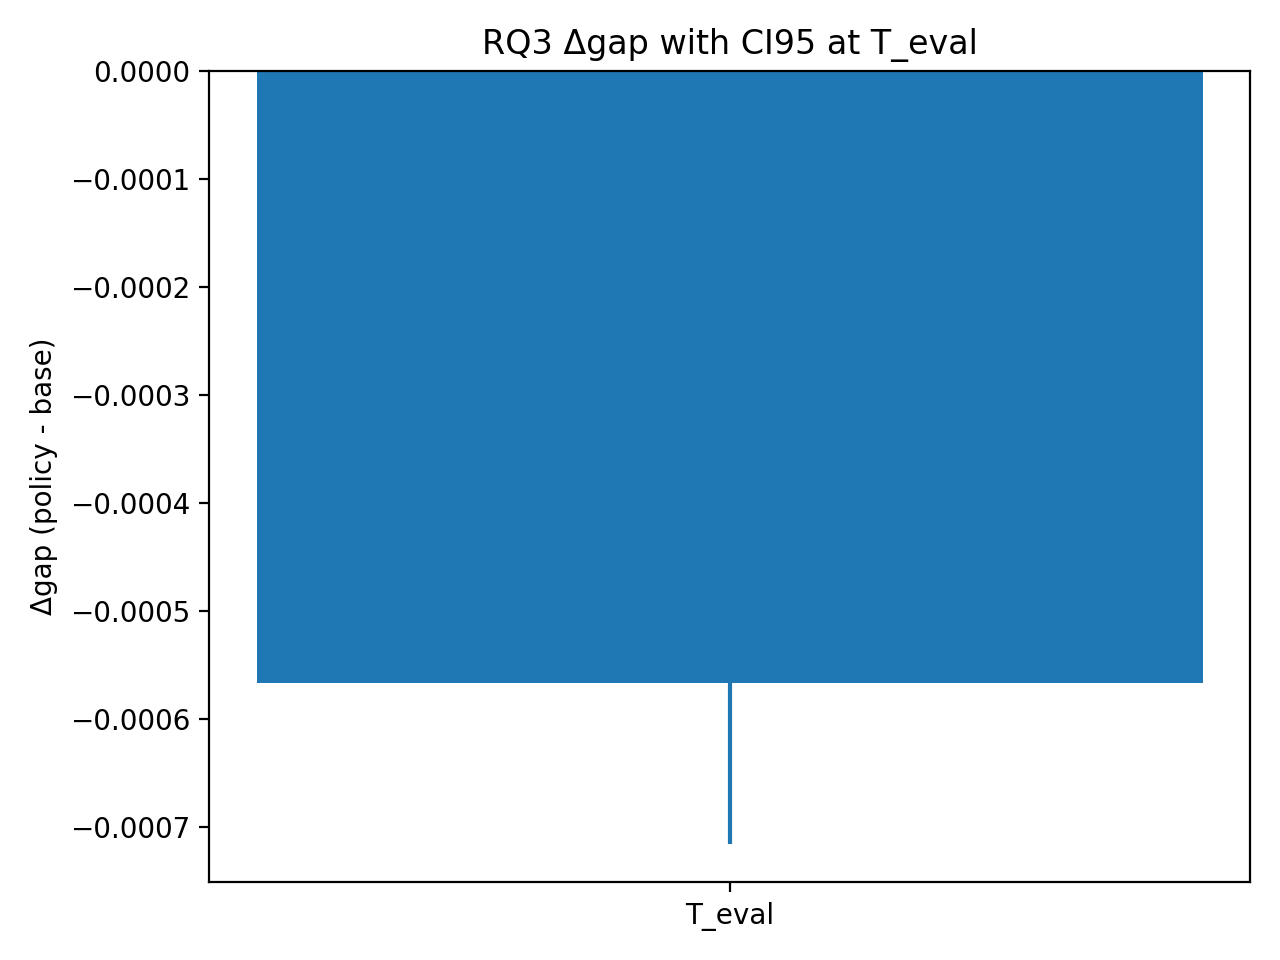
\includegraphics[width=0.45\textwidth]{outputs_v2/figures/fig_rq3_gap_Teval.png}
\caption{RQ3 gap result at $T_{eval\_metrics}=37$. Consistency with $T_{policy}$ is part of the robustness readout.}
\label{fig:rq3_gap_teval}
\end{figure}

\begin{table}[!t]
\centering
\caption{RQ3 summary with bootstrap uncertainty.}
\label{tab:rq3_summary}
\begin{tabular}{lcc}
\hline
Horizon & $\Delta Gap(T)$ & 95\% bootstrap CI \\
\hline
$T_{policy}=18$ & $-0.00050816$ & $(-0.00066222,\,-0.00032944)$ \\
$T_{eval\_metrics}=37$ & $-0.00056691$ & $(-0.00071529,\,-0.00040728)$ \\
\hline
\end{tabular}
\end{table}

Both intervals exclude zero, so the direction is robust at both horizons for the reported scenario.

\paragraph*{RQ3 conclusion.}
The framework answers RQ3 positively at the level it proposes: it can quantify subgroup-sensitive structural contrasts and attach uncertainty to their directional interpretation. This supports the use of the subgroup track as an auditable extension of the policy-simulation framework rather than as a separate fairness model.

\subsection{Results Synthesis: What the Paper Set Out to Answer}
\label{subsec:results_synthesis}

The paper set out to move from static prediction---who is at risk---to a temporal, decision-oriented framework that addresses when to act and how to compare explicit regimes. The empirical evidence supports that objective in four direct points:

\begin{enumerate}
\item Weekly hazard quality is sufficient for temporal decision support (RQ1).
\item Regime comparison is operational and auditable through $\Delta S(t)$ (RQ2).
\item The same policy can be audited for subgroup differentials via $\Delta Gap(T)$ (RQ3).
\item The main interpretation remains directionally coherent under benchmark and robustness axes.
\end{enumerate}

These are framework-validation claims under explicit scenario rules. They are not causal claims about real interventions in OULAD.

\subsection{Interpretation Boundaries}

To prevent overclaim, the results are interpreted under three explicit limits:
\begin{itemize}
\item policy and fairness outputs are simulated regime contrasts;
\item horizon-validity constraints under censoring are binding for metric interpretation;
\item endpoint and domain-shift robustness indicate sensitivity ranges, not universal transportability.
\end{itemize}

Within these limits, the section answers the paper objective directly: a reproducible temporal pipeline can translate weekly risk into explicit, auditable policy and subgroup diagnostics.
\appendices
\section{Appendix A: Supplementary Diagnostics Supporting the Core Claims}
\label{app:a}

This appendix is intentionally compact and retains only diagnostics that are most directly tied to the paper objective: translating temporal risk into auditable structural policy and subgroup diagnostics. It does not introduce new estimands, new policy regimes, or causal claims.

\subsection{Selection Rule for Supplementary Figures}

A figure is included in Appendix~A only if it satisfies at least one of the following conditions:
\begin{itemize}
\item it explains a key magnitude pattern reported in the main text;
\item it audits uncertainty for a reported structural contrast.
\end{itemize}

This rule keeps the appendix supportive rather than exploratory.

\subsection{A.1 Mechanism Diagnostics for the Policy Contrast}
\label{app:a_policy_mechanism}

The main text reports that the shock regime yields a substantially larger $\Delta S$ than the mechanism-aware regime under the default configuration. Figure~\ref{fig:app_policy_cov_deltas} is retained because it explains that difference mechanistically by showing the weekly covariate deltas induced by policy propagation.

\begin{figure}[!t]
\centering
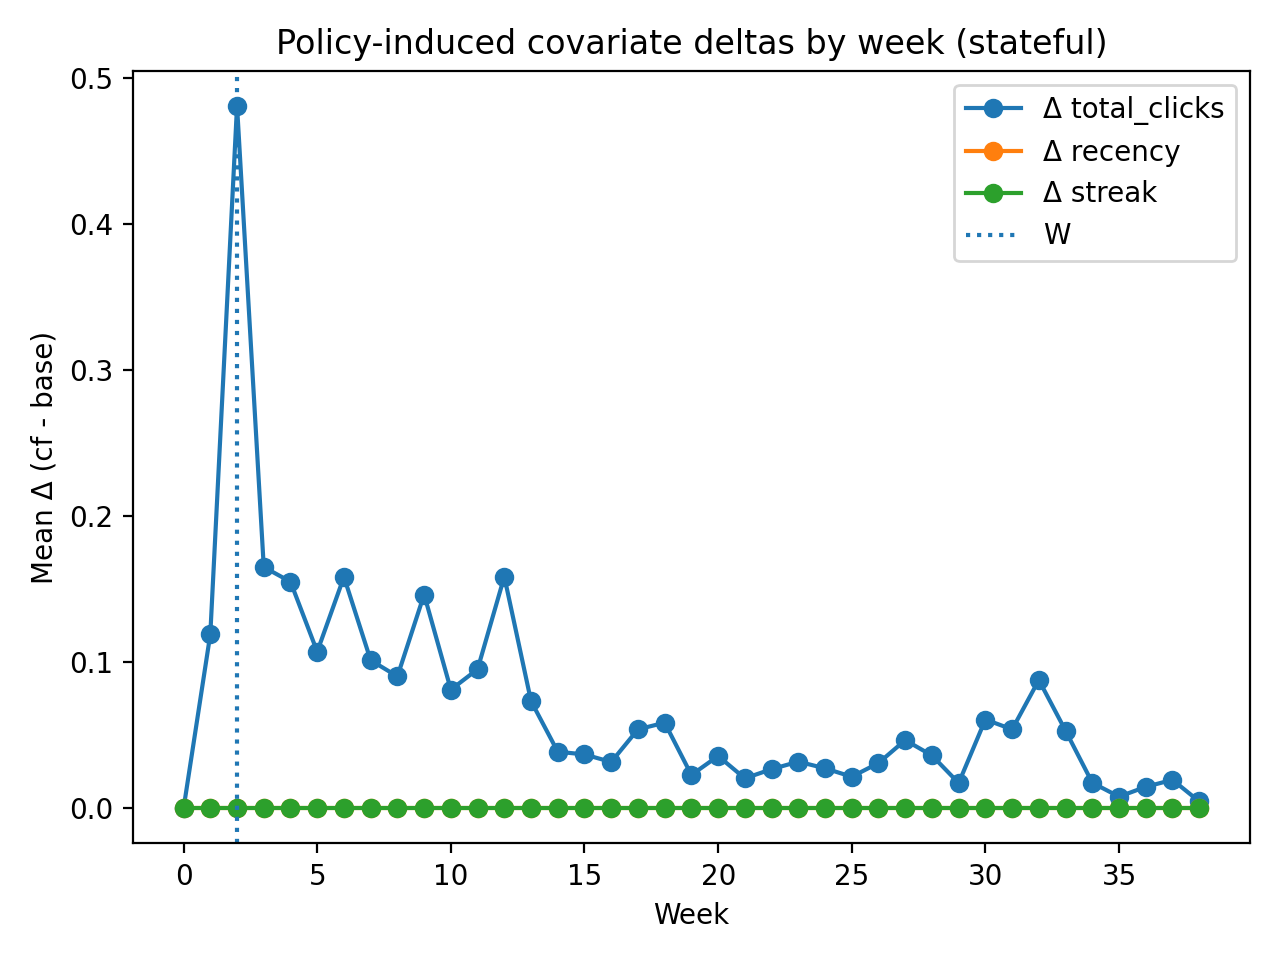
\includegraphics[width=0.45\textwidth]{outputs_v2/figures/fig_policy_covariate_deltas_by_week.png}
\caption{Supplementary mechanism diagnostics: weekly policy-induced covariate deltas. Small or short-lived deltas are consistent with weak mechanism-aware contrasts at $T_{policy}$ and negative mechanism-aware contrasts at $T_{eval\_policy}$ in the exported run.}
\label{fig:app_policy_cov_deltas}
\end{figure}

The associated numeric summaries are reported in the
\texttt{outputs\_v2/tables} artifact folder, specifically in
\texttt{table\_policy\_covariate\_deltas\_by\_week.csv}
and
\texttt{table\_policy\_activation\_summary.csv}.
This block is included because it strengthens interpretability: it shows how the simulated intervention propagates through the state variables and why the resulting structural contrast remains small in the mechanism-aware case.

\subsection{A.2 Bootstrap Uncertainty Audit for RQ3}
\label{app:a_rq3_bootstrap}

Figure~\ref{fig:app_boot_tp} is retained because it audits the stability of the subgroup change-in-gap signal reported for RQ3 at the primary horizon.

\begin{figure}[!t]
\centering
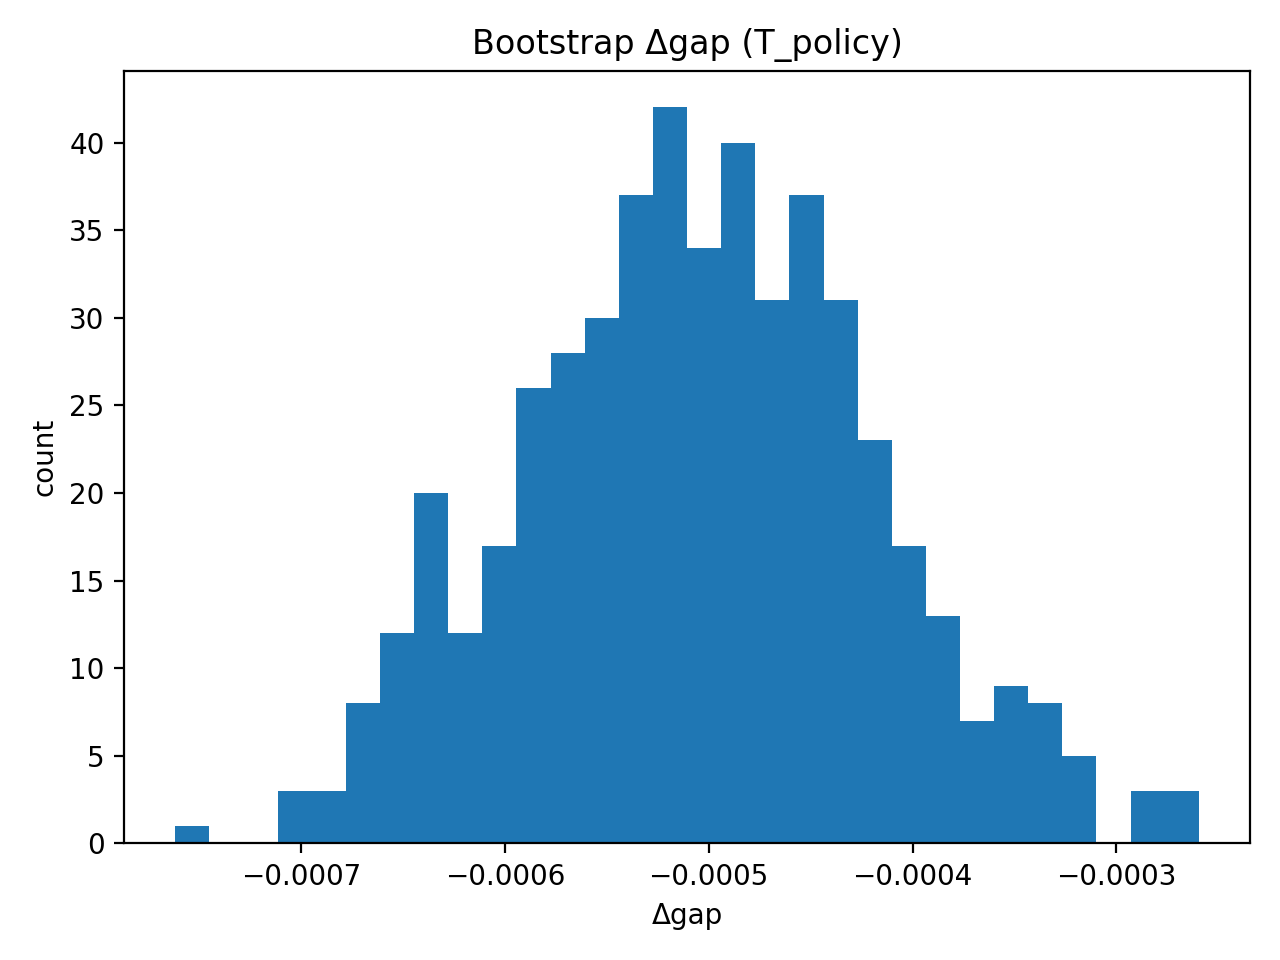
\includegraphics[width=0.45\textwidth]{outputs_v2/figures/fig_rq3_bootstrap_hist_deltagap_Tpolicy.png}
\caption{Bootstrap distribution of $\Delta Gap(T_{policy})$. Included to audit uncertainty for the subgroup contrast at the primary reporting horizon.}
\label{fig:app_boot_tp}
\end{figure}

The compact confidence-interval summaries are reported in
\texttt{rq3\_policy\_bootstrap\_wide.csv}, available in the
\texttt{outputs\_v2/tables} artifact folder, including both $T_{policy}$ and $T_{eval\_metrics}$ summaries. This block does not introduce a new subgroup result; it makes uncertainty auditing explicit.

\subsection{A.3 Appendix Boundary}

Appendix~A is intentionally constrained to diagnostics with the highest relevance to the core argument. Additional diagnostics (for example, IPCW calibration robustness and calibration-by-group) remain available in the exported artifact package under \texttt{outputs\_v2/figures} and \texttt{outputs\_v2/tables}, but are omitted here to keep the appendix focused.

Accordingly, all conclusions remain within the same contract used throughout the paper: the reported quantities are \textit{model-implied simulated regime contrasts} under explicit protocol rules, and the appendix serves only to strengthen the evidentiary basis for reading those contrasts.
\section{Appendix B: Reproducibility and Code Availability}
\label{app:b}

All experiments reported in this paper were executed through the project notebook
\texttt{TCM-Student-Dropout\_updated.ipynb} and its exported artifact workflow.
The complete source code and the notebook used to reproduce preprocessing,
temporal split construction, model training/calibration,
policy simulation, subgroup diagnostics, and artifact export are available at
\url{https://github.com/rafa-rodriguess/TCM-Student-Dropout}
\cite{RafaRepoTCMStudentDropout}.

The repository includes instructions to regenerate the exported artifacts
from raw OULAD inputs, including the full \texttt{outputs\_v2} package.
This package contains both \texttt{outputs\_v2/figures} and
\texttt{outputs\_v2/tables}, and all figures and tables referenced in the paper
correspond to files produced by this export process.

The pipeline records artifact provenance during export,
along with key protocol decisions such as split settings,
random seeds, and scenario parameters.
In particular, the reported policy and horizon settings are explicitly tracked,
including $r^*=1$, weekly checking frequency, $W=2$,
a scenario-indexed shock catalog ($\delta_{\mathrm{shock}}\in\{0.08,0.20,0.60\}$ with anchored and hypothetical statuses),
the shared mechanism-aware schedule (week-0 uplift $0.35$, week-1 uplift $0.10$),
the reference scenario identifier used for legacy-compatible outputs,
and the dual-horizon evaluation rule
($T_{policy}=18$, $T_{eval\_metrics}=37$, with
$T_{eval\_policy}=38$ as raw support horizon).

The scenario contract and its traceability fields are exported in
\nolinkurl{table_policy_scenarios_main.csv},
\nolinkurl{table_policy_scenario_params.csv},
\nolinkurl{table_policy_deltaS_by_week_by_scenario.csv}, and
\nolinkurl{table_policy_deltaS_at_horizons_by_scenario.csv}.

For the current manuscript, \texttt{outputs\_v2} is the canonical evidence package, and reported numerical results are aligned to that export set.

Reproducibility is defined at the level of the specified pipeline: the same raw inputs, protocol settings, and export workflow produce the evidence package used in this manuscript.

\section*{AI Disclosure}
Generative AI tools were used for language assistance (translation and wording
suggestions) and for brainstorming/editing support.
No generative AI was used to generate the study data, analyses,
results, or conclusions.
All manuscript content was reviewed and approved by the authors.

\bibliographystyle{IEEEtran}
\bibliography{ref}

\end{document}